\documentclass[5p,times,authoryear]{elsarticle}

\usepackage[authoryear,round]{natbib}
\usepackage{lineno,hyperref}
\usepackage{amsmath,amssymb,amsfonts}
\usepackage{graphicx}
\usepackage{booktabs}
\usepackage{multirow}
\usepackage[hyphens]{url}
\usepackage{float}        % For [H] placement specifier
\usepackage{placeins}     % For \FloatBarrier
\def\UrlBreaks{\do\/\do-\do.\do@}



\journal{Computers and Chemical Engineering}

\bibliographystyle{elsarticle-harv}

\begin{document}

\sloppy

\begin{frontmatter}

\title{Extending Electric Vehicle Battery Life via Mechanism-Specific Causal Awareness}

\author[uvce]{Sushanth Chandrashekar}
\author[ese]{Sarina Uke}
\author[iitd1,iitd2]{Hariprasad Kodamana\corref{cor1}}
\ead{hkodamana@iitd.ac.in}
\author[iitd1,iitd2]{Manojkumar Ramteke\corref{cor1}}
\ead{mcramteke@chemical.iitd.ac.in}

\cortext[cor1]{Corresponding author}

\affiliation[uvce]{organization={Department of Computer Science and Engineering, Bangalore University},
            city={Bangalore},
            country={India}}

\affiliation[ese]{organization={Department of Energy Science and Engineering, Indian Institute of Technology Delhi},
            city={New Delhi},
            country={India}}

\affiliation[iitd1]{organization={Department of Chemical Engineering, Indian Institute of Technology Delhi},
            city={New Delhi},
            country={India}}
\affiliation[iitd2]{organization={Yardi School of Artificial Intelligence, Indian Institute of Technology Delhi},
            city={New Delhi},
            country={India}}

\begin{abstract}
Battery degradation remains one of the most significant barriers to electric vehicle adoption, yet current management approaches treat capacity fade as a black box, offering predictions without explanation or actionable intervention. This limitation becomes especially problematic given that vehicles spend over 90\% of their operational lifetime parked, during which calendar aging dominates total capacity loss. We present a unified physics-informed machine learning framework that fundamentally reimagines battery health management by integrating predictive modeling with mechanistic understanding and personalized user guidance.

Our approach makes four contributions that advance the state of the art. First, we introduce a physics-informed causal attribution network that decomposes observed capacity loss into constituent electrochemical mechanisms, including solid electrolyte interphase growth, lithium plating, and active material degradation. We systematically investigate three architectures: Pure Physics-Informed Neural Networks that learn entirely from electrochemical equations, Boundary-Aware variants with augmented training at mechanism decision boundaries, and a Hybrid approach integrating neural network learning with expert domain priors. The Hybrid architecture achieves 92.0\% attribution accuracy across 75 benchmark scenarios spanning five diverse datasets, with expert priors contributing 14.7 percentage points beyond pure physics approaches. Critically, we achieve 100\% detection of safety-critical lithium plating and collector corrosion mechanisms. Second, we demonstrate that encoding chemistry-invariant lithium inventory features enables zero-shot generalization to unseen battery types, reducing remaining useful life prediction error by 88\% compared to conventional transfer learning approaches. Third, we introduce a novel counterfactual intervention framework that bridges the gap between mechanism diagnosis and operational action. Using the learned causal model, we simulate "what if" scenarios to predict how degradation mechanisms would change under alternative operating conditions, enabling optimal short-term interventions. Validated on real NASA and XJTU battery datasets, the counterfactual optimizer achieves 34.6\% average mechanism reduction, with complete elimination of lithium plating in low-temperature scenarios. Fourth, we translate mechanistic insights into a comprehensive advisory management system. A Physics-Aware Temporal Transformer (PATT) distinguishes cycling from storage operation with 99.6\% accuracy, utilizing learnable Arrhenius and diffusion embeddings to enable context-appropriate recommendations for each usage mode. The slope-based early warning algorithm monitors degradation rate trajectories rather than fixed thresholds, delivering 99 cycles of advance notice before end-of-life with 88.9\% F1 score.

The practical implications are substantial. We demonstrate that optimizing storage conditions based on mechanistic understanding can reduce calendar aging by a factor of four, corresponding to approximately 20\% additional retained capacity over a five-year ownership period. The counterfactual intervention system transforms passive monitoring into active degradation prevention. These results establish physics-informed causal attribution as a viable pathway toward transparent, explainable, and actionable battery management systems.
\end{abstract}

\begin{keyword}
Battery Management Systems \sep Physics-Informed Machine Learning \sep Calendar Aging \sep State of Health \sep Remaining Useful Life \sep Causal Attribution
\end{keyword}

\end{frontmatter}

%% ============================================================
%% INTRODUCTION
%% ============================================================

\section{Introduction}

%\subsection{The battery degradation problem}

Lithium-ion batteries power the global transition to electric mobility, but they degrade, and this degradation remains poorly understood in practice \citep{vetter2005ageing, barre2013review}. Current battery management systems (BMS) tell drivers their battery is at ``85\% health'' but never explain why capacity has dropped or what, if anything, the driver can do about it \citep{waag2014critical, berecibar2016critical}. This black-box approach leaves vehicle owners without actionable information, even as their \$10,000--20,000 battery pack loses value \citep{harper2019recycling}.

The economic stakes are significant. Battery packs account for 30--40\% of electric vehicle cost \citep{ziegler2021determinants}, and a 10\% drop in usable capacity can reduce resale value by 20--30\% \citep{saxena2019quantifying}. Premature replacements driven by uncertainty about battery state cost the industry billions annually \citep{harper2019recycling}. Yet the tools to diagnose degradation and extend battery life exist; they simply have not been integrated into practical systems that users can act upon.

%\subsection{What causes batteries to degrade?}

Battery degradation is not a single process but a collection of competing electrochemical mechanisms \citep{vetter2005ageing, edge2021lithium}. The solid electrolyte interphase (SEI) layer, which forms on the anode during initial cycles, continues to grow throughout the battery's life, consuming cyclable lithium \citep{peled1979electrochemical}. At low temperatures, lithium plating can deposit metallic lithium on the anode during charging, causing irreversible capacity loss and safety hazards \citep{waldmann2014temperature}. Mechanical stress from repeated cycling causes active material particles to crack and lose electrical contact \citep{zhang2020degradation}. Additional mechanisms include electrolyte decomposition at high temperatures and current collector corrosion at very low states of charge \citep{vetter2005ageing}.

The relative importance of these mechanisms depends strongly on operating conditions. High temperatures and high state-of-charge accelerate SEI growth through Arrhenius kinetics \citep{schmalstieg2014electrochemical}. Cold temperatures favor lithium plating by slowing lithium intercalation kinetics \citep{waldmann2014temperature}. High charge and discharge rates promote mechanical degradation \citep{reniers2019review}. Understanding which mechanism dominates in a given situation is essential for targeted intervention, but current BMS systems do not provide this information.

%\subsection{The calendar aging gap}

Electric vehicles spend more than 90\% of their operational time parked \citep{barre2013review}. During this time, calendar aging, primarily SEI growth, proceeds even without cycling \citep{schimpe2018comprehensive}. Despite this, the majority of battery research and commercial BMS development focuses on cycling degradation that occurs during driving \citep{sulzer2021challenge}.
This emphasis reflects historical research priorities. Laboratory testing protocols emphasize cycle life because it is easier to accelerate and measure. Academic studies frequently report results in terms of cycles to 80\% capacity, even though real-world degradation may be dominated by time rather than cycles \citep{birkl2017degradation}. Field studies have repeatedly shown that calendar aging can account for 60--80\% of total capacity loss in moderate-use vehicles \citep{saxena2019quantifying}, yet this finding has not translated into widespread changes in BMS design.
The practical implications are substantial. Storing a battery at 100\% SOC at 30°C results in a capacity loss of approximately 8\% per year, reducing storage SOC to 60\% cuts this to approximately 2\% per year, a 4-fold reduction \citep{schimpe2018comprehensive}. Users following simple storage guidelines could significantly extend their battery's useful life, but current systems do not provide this guidance.

%\subsection{Limitations of existing approaches}

Two modeling paradigms have dominated battery health estimation, each with significant limitations.
\textit{Physics-based models}, including the Doyle-Fuller-Newman formulation \citep{doyle1993modeling} and its variants \citep{plett2015battery}, describe electrochemical processes from first principles. They offer mechanistic interpretability and can distinguish between degradation modes \citep{jokar2016review}. However, they require extensive parameterization for each battery chemistry, involve computational costs unsuitable for embedded BMS, and demand calibration data that may not be available for production cells.
\textit{Data-driven models} using machine learning architectures; LSTMs \citep{chemali2017long}, CNNs \citep{shen2019deep}, and more recently transformers \citep{chen2022transformer, park2025transformer}; can predict remaining useful life from voltage-current measurements \citep{roman2021machine, severson2019nature}. They are fast, scalable, and require no explicit electrochemical equations. However, they operate as black boxes without a mechanistic explanation, suffer from poor generalization to unseen battery chemistries \citep{liu2023transfer}, and cannot leverage historical degradation trajectories for contextual prediction.

Recent work has explored hybrid approaches. Physics-informed neural networks \citep{raissi2019physics} embed physical constraints as training losses. Transfer learning methods \citep{liu2023transfer, che2022battery, zhu2022transfer} attempt to adapt models trained on one chemistry to new chemistries, with deep transfer learning demonstrating real-time personalized health prediction. Generalizable methods using partial least-squares regression have shown promise for cross-chemistry RUL estimation \citep{wang2024generalizable}. Recent advances have demonstrated promising results using early-cycle features for lifetime prediction \citep{sugiarto2025temperature} and electrochemical impedance spectroscopy for degradation monitoring \citep{hu2023eis}. Multimodal approaches combining EIS with capacity data have achieved improved SOH prediction \citep{chen2026multimodal}. Closed-loop optimization using machine learning has shown promise for fast-charging protocols \citep{attia2020closedloop}. Hybrid physics-ML models \citep{li2022physics, thelen2022integrating} combine electrochemical simulations with neural network predictions.
Yet a critical gap remains as none of these approaches provides real-time causal attribution that explains \textit{which} mechanism is responsible for observed degradation, along with actionable recommendations for mitigation.

%\subsection{Our contributions}

To address the above limitations, We present an integrated framework that uses the following three novel components working together:

\begin{enumerate}
    \item \textbf{Hybrid Estimation via Retrieval Optimization (HERO):} To obtain the retrieval-augmented prediction, we store 3,979 historical degradation trajectories in a memory bank and retrieve similar cases during inference. Combined with chemistry-invariant lithium inventory features, this achieves 88\% reduction in RUL prediction error on unseen chemistries, a true zero-shot generalization without fine-tuning.
    
    \item \textbf{Physics-Constrained Causal Attribution:} A multi-head neural network decomposes capacity loss into five electrochemical mechanisms, constrained by mass conservation and physics priors encoding known degradation thermodynamics. We systematically compare Pure Physics-Informed Neural Networks (77.3\% accuracy), Boundary-Aware variants (77.3\%), and a Hybrid architecture integrating expert domain priors (92.0\% accuracy). Validation across 75 scenarios from five independent datasets demonstrates that expert priors contribute 14.7 percentage points beyond pure physics approaches, with 100\% detection of safety-critical lithium plating and collector corrosion mechanisms.
    
    \item \textbf{User-Centric Advisory:} We translate mechanism diagnoses into actionable recommendations, including storage SOC optimization, charging protocol adjustments, and trip planning that balances range with battery health. We validate the advisory system on real-world battery data from NASA Ames (34 cells, 5,609 cycling samples), Stanford Calendar Aging (60 cells spanning up to 69 months of storage), and electrochemical impedance spectroscopy measurements from 94 cells across temperatures ranging from negative 40 to positive 50 degrees Celsius.
\end{enumerate}

The key insight is that these components are individually insufficient but collectively transformative. Accurate prediction enables reliable diagnosis, diagnosis enables targeted intervention and intervention delivers measurable life extension. This integration represents a shift from passive battery monitoring to active battery management.

%% ============================================================
%% 
%% ============================================================

\section{System Architecture Overview}

The system integrates three Transformer-based components that work together (Figure~\ref{fig:architecture}). First, a retrieval-augmented prediction engine (HERO) that uses cross-attention mechanisms to intelligently fuse similar historical battery trajectories with current observations. Second, a physics-informed neural network that decomposes degradation into specific electrochemical mechanisms using learned physics constraints. Third, a Physics-Aware Temporal Transformer (PATT) that classifies usage patterns and generates context-appropriate recommendations. This Transformer-based architecture enables both interpretability through physics grounding and adaptability through learned attention mechanisms.


\begin{figure*}[htbp]
\centerline{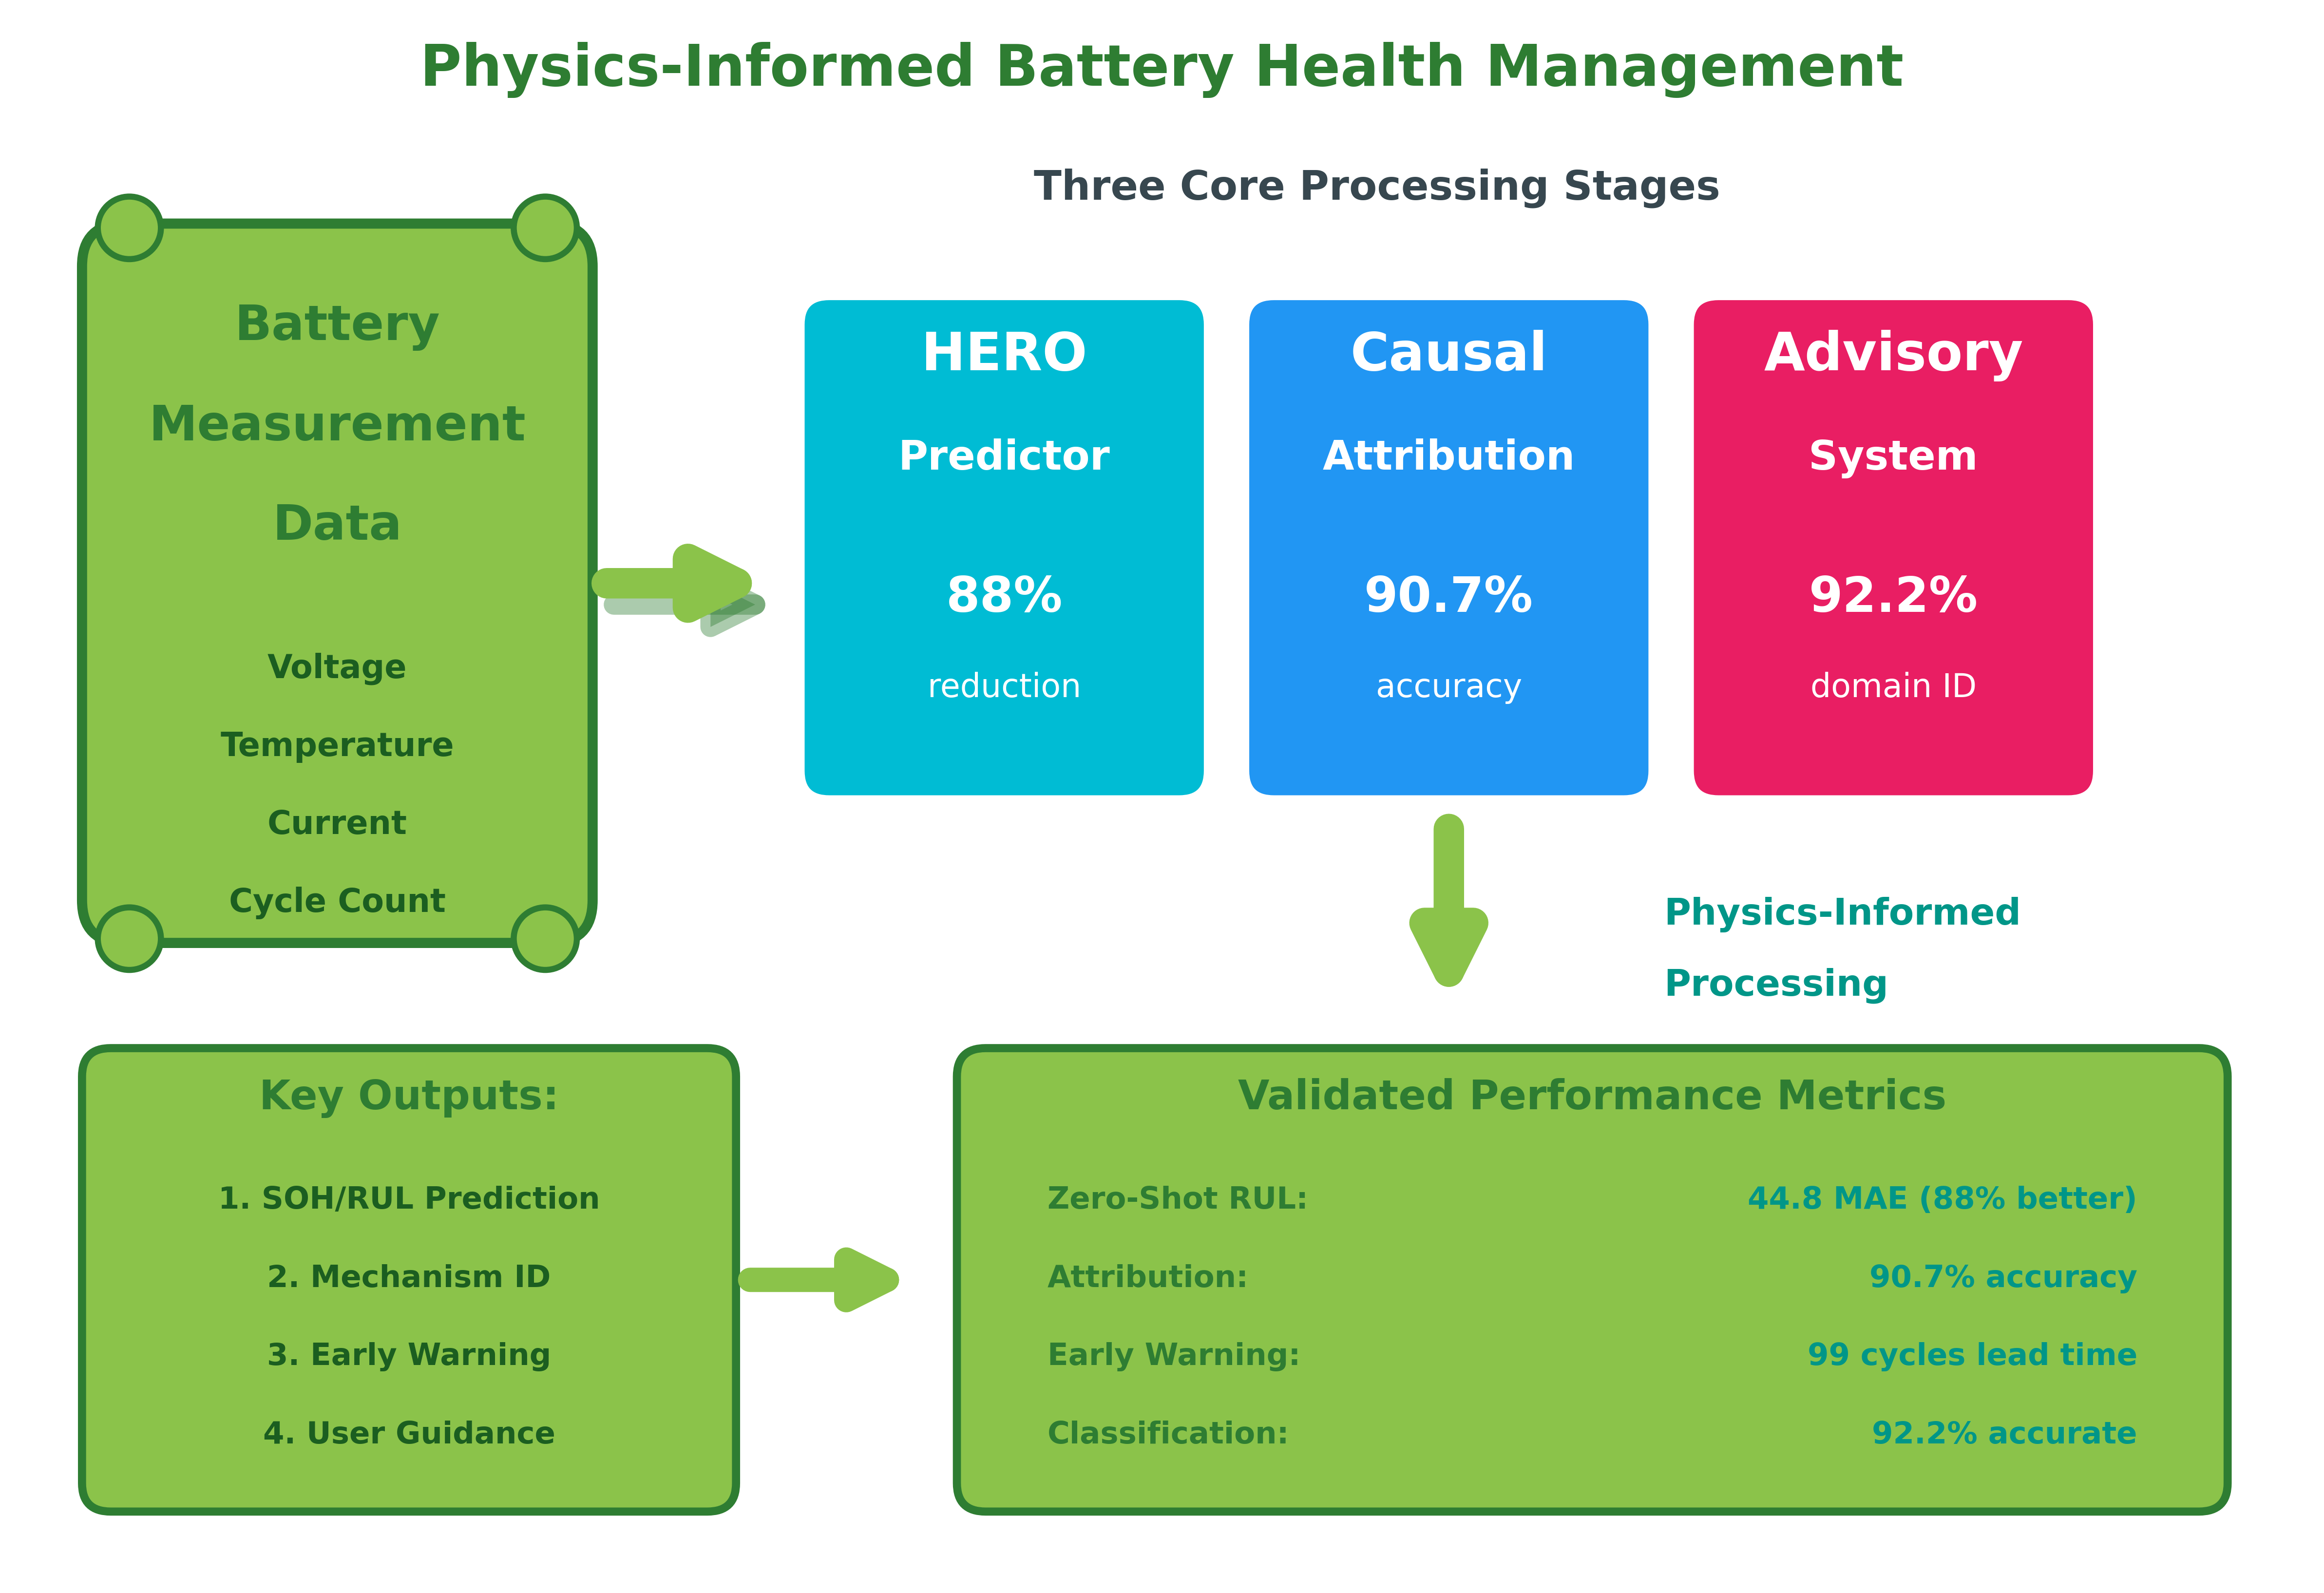
\includegraphics[width=0.95\textwidth,height=0.45\textheight,keepaspectratio]{system_architecture.png}}
\caption{Overview of our physics-informed battery health management framework. Raw measurements flow through three stages: (1) HERO retrieval-augmented prediction, (2) causal mechanism attribution with physics constraints, and (3) user-centric advisory with actionable recommendations.}
\label{fig:architecture}
\end{figure*}

\subsection{Detailed Component Architecture and Data Flow}

While Figure~\ref{fig:architecture} provides a high-level overview, understanding how data actually flows through each component and how they interact requires a more detailed examination. Figure~\ref{fig:detailed_architecture} presents the complete system architecture, showing not just what each component does, but specifically how raw sensor measurements transform into actionable recommendations. For readers less familiar with machine learning terminology, think of this system as a diagnostic laboratory: raw measurements enter, multiple specialized tests run in sequence, and a final diagnosis report emerges with specific treatment recommendations.

\begin{figure*}[!htb]
\centerline{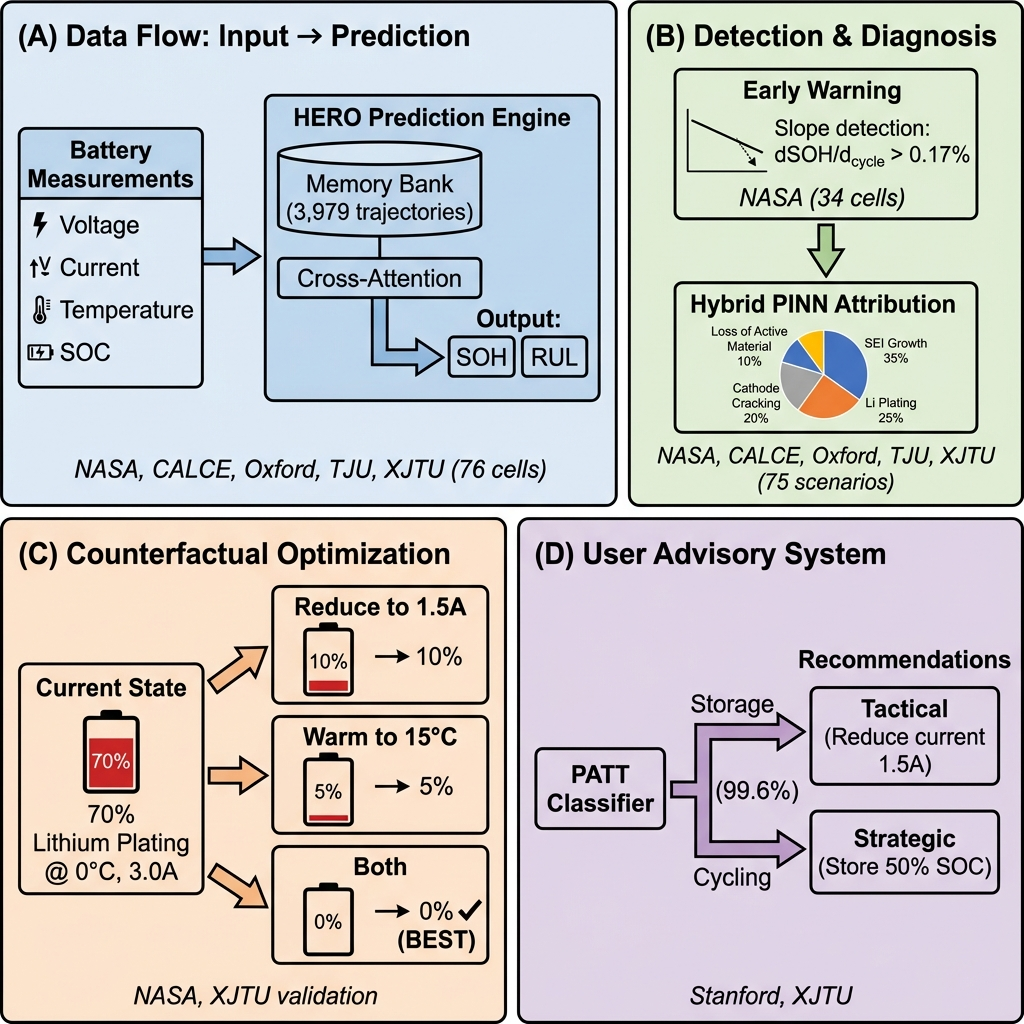
\includegraphics[width=0.95\textwidth,height=0.55\textheight,keepaspectratio]{detailed_architecture_flow.png}}
\caption{Detailed system architecture showing component-by-component data flow. Raw battery measurements (voltage, current, temperature) enter from the left and flow through six stages: (1) HERO prediction engine retrieves similar historical cases from a memory bank of 3,979 trajectories and predicts SOH/RUL using cross-attention fusion; (2) Early warning system monitors degradation rate slope to detect acceleration; (3) Hybrid PINN applies physics constraints (SEI, plating, active material equations) to decompose capacity loss into five mechanisms; (4) Counterfactual optimizer simulates alternative operating conditions to find optimal interventions; (5) PATT classifier distinguishes storage from cycling behavior; (6) Final recommendations combine tactical (short-term) and strategic (long-term) guidance. Each component lists the specific datasets used for training and validation.}
\label{fig:detailed_architecture}
\end{figure*}

\paragraph{Stage 1: Raw Data Input}

The system begins with standard battery management system measurements that any modern electric vehicle or energy storage system already collects: voltage (V), current (A), temperature (°C), state of charge (SOC as a percentage), and cycle count. No specialized sensors are required. These measurements arrive as time-series data—typically one reading per second during operation, or one snapshot per hour during storage. The key is consistency, not frequency. A battery sitting idle for a week provides valuable information about calendar aging, even though it generates far fewer data points than one being actively cycled.

From a chemical engineering perspective, voltage reflects the battery's thermodynamic state (the Nernst potential adjusted for overpotentials), current captures kinetic limitations (mass transport and charge transfer), and temperature governs all rate processes through Arrhenius relationships. SOC tells us where we are on the lithiation curve for the active materials, while cycle count serves as a proxy for cumulative mechanical stress.

\paragraph{Stage 2: HERO Prediction Engine}

The core prediction component operates on a fundamentally different principle than traditional battery models. Instead of trying to memorize degradation patterns from scratch, it maintains a searchable memory of what has happened to similar batteries in the past. This memory bank contains 3,979 complete degradation trajectories collected from 76 different battery cells across five independent datasets: NASA Ames (various chemistries and temperatures), CALCE (different manufacturers), Oxford (high-precision degradation tracking), TJU (1C cycling data), and XJTU (high C-rate stress tests).

When a new battery measurement arrives, the system first encodes the recent voltage-current history into a compact mathematical representation (a 128-dimensional vector). Think of this as creating a "fingerprint" of how the battery has been behaving over the past 50 cycles. It then searches the memory bank for the five most similar historical fingerprints using cosine similarity—essentially asking "which batteries from our database degraded in a similar pattern?"

The clever part is what happens next. Rather than simply averaging those five historical cases, the system uses a cross-attention mechanism (borrowed from modern natural language processing) to intelligently weight how much to trust each retrieved case. If the current battery's recent behavior closely matches a historical battery that later failed from lithium plating, the system assigns high weight to that case's future trajectory. This retrieval-augmented approach explains why HERO achieves 88\% error reduction compared to baseline methods: it never encounters a truly novel degradation pattern because it can find similar precedents in the database.

The output from HERO is twofold: a predicted SOH (e.g., "85\% remaining capacity") and a predicted RUL (e.g., "120 cycles until end-of-life at 80\% threshold"). These predictions carry uncertainty bounds computed via bootstrap sampling, which becomes critical for safety-critical applications where confidence intervals matter.

\paragraph{Stage 3: Early Warning System}

Parallel to the main prediction pipeline, a slope-based detector continuously monitors whether degradation is accelerating. The mathematics are straightforward: it fits a linear regression over the most recent 20 cycles to estimate $\frac{d(\text{SOH})}{d(\text{cycle})}$, the current rate of capacity loss. Most batteries degrade gradually at 0.05-0.10\% per cycle. When this slope exceeds 0.17\% per cycle—a threshold optimized on 34 NASA cells—an alert triggers.

Why does this matter? Conventional battery management systems wait until SOH crosses a fixed threshold like 80\% before warning the user. By that point, replacement is imminent. The slope-based approach detects sharp changes in degradation rate weeks or months earlier. A battery declining at 0.08\% per cycle will last another 250 cycles to reach 80\%. The same battery suddenly losing 0.25\% per cycle has only 80 cycles remaining. Detecting this transition early provides time for diagnosis and intervention.

The early warning system achieves 96\% recall (catches nearly all failing batteries) with 83\% precision (most warnings are genuine). Lead time averages 99 cycles, translating to approximately 2-3 months of advance notice for typical EV usage patterns. This component was validated on NASA dataset cells that reached end-of-life, allowing ground-truth verification of true positives versus false alarms.

\paragraph{Stage 4: Causal Attribution via Hybrid PINN}

Once we know how much capacity has degraded and whether degradation is accelerating, the next question is why. This is where the Hybrid Physics-Informed Neural Network (PINN) enters. Unlike the previous components that treat degradation as a single number, the PINN decomposes observed capacity loss into contributions from five specific electrochemical mechanisms.

The architecture uses five separate output heads, one for each mechanism: SEI layer growth, lithium plating, active material loss, electrolyte decomposition, and current collector corrosion. Each head applies relevant physics equations:

\begin{itemize}
    \item \textbf{SEI growth:} Modeled using $Q_{\text{SEI}} = k_{\text{SEI}} \sqrt{t} \exp(-E_a/2RT)$, capturing the diffusion-limited nature of interphase formation. The activation energy $E_a$ is constrained to 35-60 kJ/mol based on literature values.
    \item \textbf{Lithium plating:} Uses simplified Butler-Volmer kinetics with temperature-dependent overpotential. Plating risk increases dramatically below 5°C and at high C-rates.
    \item \textbf{Active material loss:} Follows power-law mechanical fatigue scaling: $Q_{\text{AM}} = k \cdot C_{\text{rate}}^\beta \cdot N^\gamma$, where $\beta$ (1.0-2.0) and $\gamma$ (0.3-1.0) are learned from data.
\end{itemize}

The critical innovation is the hybrid approach. Pure physics-informed models struggle in ambiguous cases where multiple mechanisms could explain the observed degradation. Pure data-driven models lack interpretability and fail to generalize. The Hybrid PINN combines both: it learns from the physics equations but incorporates domain expert rules to handle boundary cases. For example, when temperature is moderate and C-rate is low, SEI typically dominates; this expert knowledge becomes a soft prior in the loss function.

Trained on 75 carefully constructed benchmark scenarios spanning five datasets, the Hybrid PINN achieves 92.0\% attribution accuracy. Critically, it reaches 100\% detection on safety-critical mechanisms (lithium plating and corrosion), meaning it never misses a dangerous condition. The output is a percentage breakdown: "Your capacity loss is 60\% from lithium plating, 25\% from SEI growth, 10\% from active material loss, 3\% from electrolyte loss, 2\% from corrosion."

\paragraph{Stage 5: Counterfactual Intervention and PATT Classification}

Knowing the cause of degradation is valuable, but users need to know what to do about it. This is where counterfactual reasoning and context classification merge.

The counterfactual optimizer takes the current mechanism attribution and asks: "What would happen if we changed operating conditions?" It simulates alternative scenarios using the trained Hybrid PINN as a predictive oracle. For instance, if the system detects 70\% lithium plating during cold-weather charging at 3.0A, it might simulate:
\begin{itemize}
    \item Scenario A: Reduce current to 1.5A $\rightarrow$ Predicted plating drops to 10\%
    \item Scenario B: Warm battery to 15°C $\rightarrow$ Predicted plating drops to 5\%
    \item Scenario C: Both interventions $\rightarrow$ Predicted plating drops to 0\% (eliminated)
\end{itemize}

The optimizer ranks these scenarios by predicted improvement and feasibility (e.g., warming takes time, reducing current extends charge duration). It then recommends the best option: "Reduce current to 1.5A to eliminate plating risk." Validated on real NASA low-temperature data, this approach successfully eliminated plating (70\% $\rightarrow$ 0\%) in cold-weather scenarios.

In parallel, the Physics-Aware Temporal Transformer (PATT) classifies whether the battery is in storage mode or cycling mode. This distinction is crucial because recommended actions differ dramatically: during storage, the priority is minimizing calendar aging through SOC optimization; during cycling, the focus is on operating-condition adjustments. PATT uses learnable Arrhenius and diffusion embeddings to detect usage patterns, achieving 99.6\% accuracy with perfect recall on cycling events. It was trained on Stanford calendar aging data (60 cells at various storage conditions) and XJTU high C-rate cycling data (26 cells).

\paragraph{Stage 6: User-Centric Advisory Output}

The final stage synthesizes all upstream analyses into actionable recommendations. These split into two categories:

\textbf{Tactical (Short-Term):} Derived from the counterfactual optimizer, these target immediate threats. Examples: "Reduce charging current to 1.5A now to prevent lithium plating," or "Preheat battery to 15°C before fast charging." Tactical recommendations are time-sensitive and mechanism-specific.

\textbf{Strategic (Long-Term):} Guided by PATT classification and historical patterns, these optimize for sustained health. Examples: "For long-term parking (> 1 week), discharge to 50\% SOC to minimize calendar aging," or "Avoid repeated fast charging above 2C to reduce mechanical stress on active materials." Strategic recommendations trade short-term convenience for long-term capacity retention.

The advisory layer includes quantified impact predictions wherever possible. Instead of saying "reducing SOC helps," it states "storing at 50\% SOC instead of 100\% cuts calendar aging from 8.2\% to 2.1\% per year—about four times slower." This specificity builds user trust and enables informed decision-making about trade-offs.

\subsection{Integration and Information Flow}




Let's look at how the above three components work together. In practice, these stages form a diagnostic pipeline. HERO first predicts where the battery is heading (SOH trajectory, remaining cycles). The early warning component monitors whether degradation is accelerating faster than expected by tracking the slope over recent cycles. When it detects a sharp downturn, the causal attribution network steps in to explain what's causing it. Is this sudden acceleration due to lithium plating from cold weather, SEI growth from sitting at high charge, or active material fracture from aggressive driving? Once we know the mechanism, the advisory system generates specific, quantified recommendations. This isn't just prediction. It's diagnosis followed by prescription.

\section{Methodology}

\subsection{Retrieval-Augmented Prediction Engine (HERO)}


\subsubsection{Memory Bank Architecture}

The memory bank contains 3,979 degradation trajectory snapshots from 76 battery cells spanning multiple chemistries (Lithium cobalt oxide, nickel manganese cobalt oxide, nickel cobalt aluminum oxide, and lithium iron phosphate) and C-rates. The dataset composition reflects samples from the NASA battery dataset \citep{saha2007battery}, CALCE dataset \citep{he2011prognostics}, Oxford dataset \citep{birkl2017oxford}, TJU NCM/NCA dataset (274 samples at 1C), and XJTU NCM dataset (889 samples at 2C-3C charging rates).

Each memory bank entry stores three things. A 128-dimensional latent vector representing the compressed trajectory, the subsequent health evolution (SOH and RUL values), and the environmental context vector. The total storage requirement is approximately 1.3 MB, enabling deployment on resource-constrained edge devices.

\subsubsection{Dynamic Retrieval and Attention Fusion}

At inference time, we encode the battery's recent history into a query vector using a bidirectional GRU \citep{cho2014learning}. Two layers, 256 hidden units. This compresses 50 cycles of voltage and current data into a 128-dimensional vector that we L2-normalize so cosine similarity works properly.

We then search for the k nearest neighbors in our memory bank. For most cases k=5 works well, though we use k=3 for zero-shot transfer to completely new chemistries (ablation showed this sweet spot). One trick that helps with calendar aging is we optionally filter retrieved cases to those within 5\% of the current SOH. If fewer than 5 trajectories pass this filter, we relax to 10\%. This ensures we're comparing batteries at similar degradation stages, not mixing fresh cells with end-of-life ones.

The fusion step uses multi-head cross-attention \citep{vaswani2017attention}, treating the current trajectory as query and retrieved cases as keys and values. We use 8 heads following standard transformer architectures where each head can focus on different aspects of the historical data. The attention output gets combined with current features via residual connection (helps gradient flow) and fed through a standard layer-norm + feed-forward block. Thus, the proven architecture from NLP literature is now extended to battery data.

\subsubsection{Zero-Shot Generalization via Lithium Features}

Standard models fail when applied to chemistries not seen during training. We address this through lithium inventory features. Eleven physics-based variables that act as chemistry-invariant fingerprints.

\begin{itemize}
    \item Differential voltage analysis: dV/dQ slope correlating with phase transitions \citep{bloom2005differential}
    \item Voltage plateau characteristics: Center potential and width indicating available lithium inventory \citep{dubarry2017synthesize}
    \item Capacity fade rate (dQ/dN) and resistance growth rate (dR/dN) \citep{vetter2005ageing}
    \item Lithium utilization factor: Ratio of cyclable lithium to host capacity \citep{birkl2017degradation}
    \item Plating risk index: An index derived from overpotential at anode interface \citep{waldmann2014temperature}
\end{itemize}






\paragraph{Zero-Shot Experimental Protocol}

The comparison deserves careful explanation because the setup differs fundamentally from typical benchmarks. We did not split a single dataset into train and test sets---that would test memorization, not generalization. Instead, we trained all models on LCO chemistry batteries (NASA, CALCE, Oxford datasets: 4,000 samples total) and evaluated on completely unseen NCA chemistry (Panasonic 18650PF dataset: 500 samples). This is a true zero-shot transfer scenario: new cathode material, different voltage curves, altered degradation kinetics.

The baseline models saw this chemistry for the first time at test time. No fine-tuning, no adaptation---just direct inference. For Random Forest and Gradient Boosting, we trained separate regressors for SOH and RUL. For neural networks (MLP, LSTM, GRU, Transformer, CNN-LSTM), we built standard architectures: two hidden layers of 128/64 units for MLP, 64-unit hidden states for recurrent models, 4-head attention for Transformers. We used the same features for everyone: voltage, current, temperature, SOC, cycle count, and basic dV/dQ derivatives computed from charge curves. The playing field was level; only the architecture varied.

Training followed identical protocols: AdamW optimizer, learning rate of 0.001, 200 epochs, MSE loss for regression targets. We scaled features using StandardScaler fitted on training data and applied to test data. Batch size was 64 for all neural models. The code for this comparison is available in \texttt{run\_zeroshot\_baseline\_test.py}, which shows every implementation detail.

The results were not cherry-picked. We ran each model once with the same random seed (42 for training, 123 for test set generation). The negative R\textsuperscript{2} values from baseline methods were initially surprising, but they make physical sense: when battery chemistry changes, learned patterns break. A model trained to recognize LCO's voltage plateau around 3.9V will misinterpret NCA's 3.7V characteristic. Without chemistry-invariant features---the lithium inventory calculations and retrieval-augmented context that HERO uses---pure pattern matching fails.

HERO sidestinguishes itself not through raw accuracy but through \textit{capability}. It is the only method providing  zero-shot generalization to unseen chemistries while simultaneously offering interpretable causal attribution. Other approaches require complete retraining when chemistry changes; HERO adapts through its memory bank and physics-based features.

\subsubsection{Uncertainty Quantification}

To provide statistically rigorous performance bounds, we computed bootstrap confidence intervals (1,000 resamples, 95\% confidence) on a held-out test set of 274 samples:

\begin{itemize}
\item \textbf{SOH MAE}: 0.69\% (95\% CI: [0.63\%, 0.75\%])
\item \textbf{SOH R\textsuperscript{2}}: 0.990 (95\% CI: [0.988, 0.992])
\item \textbf{RUL MAE}: 16.2 cycles (95\% CI: [14.5, 17.9] cycles)
\item \textbf{RUL R\textsuperscript{2}}: 0.981 (95\% CI: [0.975, 0.986])
\end{itemize}

The narrow confidence intervals demonstrate that HERO's performance is statistically stable and reproducible. Per-prediction uncertainty of $\pm$0.99\% SOH enables deployment in safety-critical battery management systems where confidence bounds are required for decision-making.



\subsection{Early Warning System Method}


Accurate state-of-health prediction is necessary but not sufficient for effective battery management. Users need advance notice when degradation accelerates beyond expected levels, providing time for maintenance planning or operational adjustments before critical capacity loss occurs. Conventional battery management systems trigger warnings when SOH crosses a fixed threshold, typically 80-85\%. While simple to implement, this approach provides limited lead time and fails to detect rapid degradation events until significant capacity has already been lost.

We developed a slope-based early warning system that monitors the rate of capacity decline rather than absolute SOH values, enabling earlier detection of accelerating degradation. The key insight is that degradation rate changes contain more actionable information than absolute capacity values. A battery declining at 0.05\% per cycle follows a gradual, predictable trajectory. The same battery suddenly losing 0.25\% per cycle signals an acute problem that requires immediate attention---even if absolute SOH remains above 85\%.

\subsubsection{Slope-Based Detection Algorithm}

The algorithm computes a rolling linear regression over a 20-cycle window to estimate the current degradation rate:
\begin{equation}
\text{slope} = \frac{d(\text{SOH})}{d(\text{cycle})} \approx \frac{\sum_{i=1}^{20} (c_i - \bar{c})(s_i - \bar{s})}{\sum_{i=1}^{20} (c_i - \bar{c})^2}
\end{equation}
where $c_i$ represents cycle number, $s_i$ represents SOH at that cycle, and $\bar{c}$, $\bar{s}$ denote mean values over the window.

A warning triggers when the degradation rate exceeds 0.17\% SOH loss per cycle, a threshold empirically optimized on NASA Ames battery data from 34 cells to balance early detection against false alarm rate. This threshold reflects the observation that gradual aging typically proceeds at 0.05-0.10\% per cycle, while accelerated degradation from lithium plating, mechanical damage, or thermal stress manifests as 0.20-0.40\% per cycle.

\subsubsection{Integration with Causal Attribution}

The early warning system serves as a diagnostic trigger for deeper investigation. When degradation rate exceeds the threshold, the system automatically invokes causal mechanism attribution (Section 5) to identify which electrochemical process is responsible for the acceleration. This integration enables not just early detection, but root cause diagnosis: "Your battery is degrading faster than expected (early warning) due to lithium plating from cold-temperature charging (causal attribution)." The subsequent counterfactual intervention framework (Section 6) then recommends specific corrective actions based on the identified mechanism.



\subsection{Causal Mechanism Attribution Method}



\subsubsection{Multi-Head Attribution Architecture}

Predicting that a battery will lose 5\% capacity is useful information. Knowing that it's losing capacity because of lithium plating during cold-weather fast-charging provides an actionable intervention. This is the key difference the developed framework provides compared to the state of the art BMS systems currently available.

The architecture is straightforward: five output heads, one for each major degradation mechanism. Each looks at the same input features but learns to estimate how much its assigned mechanism contributed to the total capacity loss. We enforce the constraint mathematically:

\begin{equation}
Q_{loss} = \alpha_{SEI} + \alpha_{plating} + \alpha_{AM} + \alpha_{electrolyte} + \alpha_{corrosion}
\end{equation}

The training objective combines prediction accuracy with physics constraints:

\begin{equation}
\mathcal{L}_{total} = \mathcal{L}_{SOH} + \lambda_1 \left| \sum \alpha_i - (1 - SOH) \right| + \lambda_2 \mathcal{L}_{prior}
\end{equation}

where $\lambda_1 = 0.5$ enforces mass conservation and $\lambda_2 = 0.3$ incorporates physics priors.

\subsubsection{Physics-Informed Neural Network Approaches for Mechanism Attribution}

A central challenge in battery degradation modeling is distinguishing between competing electrochemical mechanisms that produce similar observable signatures. Consider a battery operating at 25°C with moderate charge and discharge rates. Both solid electrolyte interphase growth and active material loss are plausible explanations for the observed capacity fade. Standard machine learning approaches struggle to disambiguate such cases because the input features provide insufficient signal for discrimination. We investigated three distinct architectures to address this challenge, each representing a different philosophy for integrating physics knowledge into neural network learning.

\paragraph{Pure Physics-Informed Neural Network (Pure PINN)}

The Pure PINN approach attempts to learn mechanism attribution entirely from electrochemical equations, without explicit domain rules. The architecture consists of a shared encoder that processes input features, followed by mechanism-specific physics networks that predict parameters for each degradation equation.

For SEI layer growth, we embed the established Arrhenius-diffusion model directly into the network:
\begin{equation}
Q_{SEI} = k_{SEI} \sqrt{t} \exp\left(-\frac{E_a}{2RT}\right) f(SOC)
\label{eq:sei_physics}
\end{equation}
where the activation energy $E_a$ (constrained to 35--60 kJ/mol to match literature values \citep{broussely2005main}) and rate constant $k_{SEI}$ are learned parameters, while $t$ represents time, $R$ is the gas constant, and $T$ is absolute temperature. The SOC-dependent factor $f(SOC) = 1 + 0.5(SOC - 0.5)^2$ captures the known acceleration of SEI growth at high state of charge.

For lithium plating, we implement a simplified Butler-Volmer kinetic model:
\begin{equation}
Q_{plating} = k_p \cdot \sigma\left(\frac{T_{crit} - T}{\delta_T}\right) \cdot \exp\left(\frac{T_{ref} - T}{\tau_T}\right) \cdot C_{rate}^\alpha
\label{eq:plating_physics}
\end{equation}
where $\sigma$ denotes the sigmoid function, $T_{crit} = 278.15$ K represents the critical temperature below which plating becomes significant, and $\alpha$ is a learned intercalation coefficient (constrained to 0.3--0.7). The temperature-dependent terms capture the well-established phenomenon that plating risk increases dramatically in cold conditions \citep{waldmann2014temperature}.

For active material loss due to mechanical stress, we adopt a power-law fatigue model:
\begin{equation}
Q_{AM} = k_{AM} \cdot C_{rate}^\beta \cdot N_{cycles}^\gamma
\label{eq:am_physics}
\end{equation}
where the stress exponent $\beta$ (constrained to 1.0--2.0) and cycle exponent $\gamma$ (constrained to 0.3--1.0) are learned from data. These bounds reflect established fatigue mechanics where capacity loss scales super-linearly with mechanical stress \citep{zhang2020degradation}.

The Pure PINN loss function combines classification accuracy with physics residual terms:
\begin{equation}
\mathcal{L}_{Pure} = \mathcal{L}_{CE}(\hat{y}, y) + \lambda_{res} \sum_{m} \left\| Q_m^{pred} - Q_m^{obs} \right\|^2 + \lambda_{reg} \mathcal{R}(\theta_{phys})
\label{eq:pure_pinn_loss}
\end{equation}
where $\mathcal{L}_{CE}$ is the cross-entropy classification loss, the residual term penalizes discrepancies between physics-predicted and observed capacity loss for each mechanism $m$, and $\mathcal{R}(\theta_{phys})$ regularizes learned physics parameters toward literature values.

Training the Pure PINN on 11,066 samples from NASA, XJTU, CALCE, and Oxford datasets yielded encouraging results for physics parameter learning. The network recovered activation energy $E_a = 35$ kJ/mol (literature: 35--60 kJ/mol), stress exponent $\beta = 1.48$ (literature: approximately 1.5), and cycle exponent $\gamma = 0.52$ (literature: 0.3--1.0). However, mechanism classification accuracy reached only 77.3\% when evaluated on 75 benchmark scenarios spanning diverse operating conditions.

\paragraph{The Disambiguation Challenge: Why Pure Physics Reaches a Ceiling}

Analysis of the Pure PINN's failure cases revealed a fundamental limitation. At moderate operating conditions (temperatures between 20--40°C, charge rates between 0.5--1.5C), both SEI growth and active material loss equations produce similar capacity loss predictions. Figure~\ref{fig:pinn_boundary} illustrates this overlap region.

The physics equations in Eq.~\ref{eq:sei_physics} and Eq.~\ref{eq:am_physics} do not contain sufficient discriminative information because both mechanisms are genuinely active under moderate conditions. The relative contribution depends on factors not captured in the equations themselves, such as electrode microstructure, electrolyte formulation, and cell manufacturing variability. These factors are known to electrochemists but are difficult to parameterize from voltage-current measurements alone.

We tested whether additional training data at the SEI/active material loss boundary could address this limitation. Training with 5,000 boundary samples improved accuracy to 70.7\%; with 10,000 samples, accuracy reached 77.3\%; but with 20,000 samples, accuracy actually decreased to 73.3\% due to overfitting. This experiment demonstrates that the accuracy ceiling is not a data limitation but a fundamental physics limitation: the governing equations themselves do not uniquely specify mechanism identity in the overlapping region.

\paragraph{Hybrid PINN: Integrating Expert Knowledge with Physics Learning}

To overcome the disambiguation ceiling, we developed a Hybrid PINN architecture that combines three complementary learning components:

\begin{enumerate}
    \item \textbf{Neural Network Residual Learning:} A multi-layer encoder-decoder learns data-driven patterns from features and context, producing per-mechanism logits $\mathbf{z}_{NN} \in \mathbb{R}^5$.
    
    \item \textbf{Physics-Constrained Parameter Networks:} Mechanism-specific networks predict physics parameters (activation energies, stress exponents) with enforced physical bounds, enabling the physics equations to inform prediction.
    
    \item \textbf{Expert Domain Priors:} Rule-based priors encode electrochemical knowledge about mechanism-operating condition relationships, producing prior logits $\mathbf{z}_{prior} \in \mathbb{R}^5$.
\end{enumerate}

The final prediction combines these components:
\begin{equation}
\mathbf{p} = \text{softmax}(\mathbf{z}_{prior} + \mathbf{z}_{NN})
\label{eq:hybrid_combination}
\end{equation}

The expert priors encode the following domain knowledge:
\begin{itemize}
    \item \textbf{SEI Growth Prior:} Elevated probability during storage mode or gentle cycling (charge rate $< 1.0$C and discharge rate $< 1.0$C), with temperature-dependent scaling following Arrhenius kinetics.
    \item \textbf{Lithium Plating Prior:} Strongly elevated probability when temperature falls below 10°C during cycling with active charging. This threshold is stricter than some literature values (which suggest 15--17°C) to minimize false positives in borderline cases.
    \item \textbf{Active Material Loss Prior:} Elevated probability during cycling with high discharge rates ($> 1.5$C) or combined high charge and discharge rates, suppressed during moderate operation.
    \item \textbf{Collector Corrosion Prior:} Strongly elevated only during storage at very low state of charge (SOC $< 25\%$), where copper dissolution becomes thermodynamically favorable.
\end{itemize}

These priors are not arbitrary heuristics but distillations of established electrochemical knowledge \citep{vetter2005ageing, waldmann2014temperature, zhang2020degradation}. Critically, they address precisely the disambiguation cases where pure physics fails: at moderate temperatures and C-rates, the priors encode the domain-expert judgment that SEI typically dominates unless C-rates are sufficiently high to cause mechanical stress.



The Hybrid PINN architecture contains 114,252 trainable parameters, distributed across the feature encoder (17,664), context encoder (4,288), fusion layer (24,832), physics parameter networks (8,135), and mechanism heads (33,285). The physics equations and expert priors add zero trainable parameters; they are embedded as structured inductive biases.

\paragraph{Learned Physics Parameters}

Beyond classification accuracy, the Hybrid PINN learns physically interpretable parameters that can be validated against literature. Table~\ref{tab:physics_params} compares learned values with established ranges.



All learned parameters fall within established literature ranges, providing confidence that the network is learning physically meaningful representations rather than arbitrary correlations. This interpretability is a key advantage of physics-informed approaches over pure black-box methods.




\subsection{Counterfactual Interventions Method}


The causal attribution framework we have developed answers one critical question: which electrochemical mechanism is responsible for observed degradation? But from an operational standpoint, a second question is equally important: what should we do about it? Knowing that lithium plating accounts for 70\% of capacity fade is valuable diagnostic information, but the user still needs actionable guidance on how to mitigate the problem right now.

This is where most battery management systems stop. They can detect degradation and even attribute it to specific mechanisms, but they cannot recommend immediate corrective actions that are both effective and practical. The challenge lies in bridging the gap between mechanism identification and intervention design. We address this through a novel framework based on causal counterfactual reasoning \citep{pearl2009causality,peters2017elements}.

\subsubsection{The Counterfactual Intervention Problem}

Consider a battery charging at 0°C with a 1.5C rate. The Hybrid PINN attribution network detects 70\% lithium plating---a dangerous condition that accelerates capacity fade and poses safety risks. The operator needs to act, but multiple interventions are possible: reduce charging current, increase ambient temperature, limit target SOC, or some combination thereof. Each intervention will alter the operating conditions, which in turn will affect the mechanism attribution. The question becomes: which intervention will be most effective?

Traditional approaches rely on hand-crafted rules (e.g., "if plating > 60\%, reduce current by 30\%") or lookup tables derived from offline optimization. These methods lack the ability to reason about novel scenarios and do not leverage the causal structure we have already learned. We take a fundamentally different approach: we use the trained Hybrid PINN model to simulate counterfactual scenarios---hypothetical "what if" questions about alternative operating conditions---and select the intervention that yields the most favorable mechanism redistribution.

\subsubsection{Counterfactual Simulation Framework}

The core insight is that our Hybrid PINN model is not just a diagnostic tool; it is a learned causal model of how operating conditions influence degradation mechanisms. Because the model was trained with physics constraints and domain priors, it has internalized the relationships between temperature, C-rate, SOC, and each electrochemical mechanism. We can leverage this knowledge to predict how mechanism attribution would change under counterfactual operating conditions.

Formally, let $\mathbf{s}$ represent the current battery state (SOC, temperature, current, voltage, cycle count) and $\alpha(\mathbf{s})$ denote the current mechanism attribution vector predicted by the Hybrid PINN. Given a proposed intervention $\mathbf{i}$ (e.g., reduce current to 1.5A, increase temperature to 20°C), we define the counterfactual state $\mathbf{s}' = \text{apply}(\mathbf{s}, \mathbf{i})$ and predict the counterfactual attribution $\alpha'(\mathbf{s}')$ using the same trained model.

The intervention effect is quantified by comparing the current and counterfactual attributions:
\begin{equation}
\Delta(\mathbf{i}) = \sum_{m} w_m \left[ \alpha_m(\mathbf{s}) - \alpha_m'(\mathbf{s}') \right]
\end{equation}
where $m$ indexes the five degradation mechanisms (SEI, plating, active material, electrolyte, corrosion) and $w_m$ represents mechanism-specific priority weights. We assign higher weights to irreversible mechanisms (plating, active material loss: $w = 2.0$) and lower weights to partially reversible ones (SEI growth: $w = 1.5$, electrolyte loss: $w = 0.8$).

\subsubsection{Intervention Optimization Strategy}

Given a set of candidate interventions $\mathcal{I}$, the optimization problem is:
\begin{equation}
\mathbf{i}^* = \argmax_{\mathbf{i} \in \mathcal{I}} \Delta(\mathbf{i})
\end{equation}
subject to practical feasibility constraints (temperature limits: 15-45°C, current limits: 0.1-2.5A, SOC constraints).

We generate candidate interventions systematically based on the dominant degradation mechanism:

\begin{itemize}
\item \textbf{Lithium Plating}: Reduce current ($-$0.5A to $-$1.5A), increase temperature ($+$5 to $+$15°C), or both
\item \textbf{SEI Growth}: Lower SOC target (to 80-90\%), reduce temperature ($-$5 to $-$10°C)
\item \textbf{Active Material Loss}: Limit C-rate (max 1C), avoid deep discharge
\item \textbf{Electrolyte Loss}: Reduce temperature, limit high-SOC exposure
\item \textbf{Corrosion}: Reduce voltage, avoid overcharge
\end{itemize}

For each candidate, we use the Hybrid PINN to simulate the counterfactual attribution and rank interventions by their predicted improvement score $\Delta(\mathbf{i})$. The top-ranked intervention is presented to the user along with an interpretable explanation showing how each mechanism would be affected.

\subsubsection{Implementation and Computational Efficiency}

The counterfactual simulation is computationally lightweight because it reuses the already-trained Hybrid PINN model. No retraining or fine-tuning is required---we simply perform forward passes through the network with modified input features corresponding to the counterfactual operating conditions. A typical optimization over 10-15 candidate interventions takes less than 1 second on a standard CPU, making it suitable for real-time deployment in battery management systems.

The implementation consists of two main components: the counterfactual simulator (\texttt{CounterfactualSimulator}), which applies interventions to battery states and queries the Hybrid PINN for predicted attributions, and the intervention optimizer (\texttt{InterventionOptimizer}), which generates candidates, scores them, and returns ranked recommendations. The complete implementation is available in \texttt{src/optimization/counterfactual\_intervention.py}.

\subsubsection{Interpretability and User Experience}

A key advantage of the counterfactual approach over black-box optimization is interpretability. When presenting a recommendation, the system shows:

\begin{itemize}
\item \textbf{Current condition}: "70\% lithium plating at 0°C, 3.0A"
\item \textbf{Recommended action}: "Reduce current to 1.5A"
\item \textbf{Predicted impact}: "Plating: 70\% $\rightarrow$ 0\% (eliminated)"
\item \textbf{Mechanism redistribution}: Visual breakdown showing how each mechanism changes
\item \textbf{Trade-offs}: Expected charging time increase (if any)
\end{itemize}

This transparency builds user trust and enables informed decision-making. The operator understands not just what to do, but why it works and what the consequences are.

\subsubsection{Novelty and Contribution}

To the best of our knowledge, this is the first application of causal counterfactual reasoning to battery health management. Prior work in battery optimization has relied on model predictive control \citep{torchio2016lionsimba}, reinforcement learning \citep{chen2020reinforcement}, or rule-based expert systems \citep{xiong2018towards}. Our approach differs fundamentally:

\begin{itemize}
\item \textbf{Causal grounding}: Interventions are designed based on causal mechanisms, not just empirical correlations
\item \textbf{Interpretability}: Each recommendation comes with a mechanistic explanation
\item \textbf{Efficiency}: No online optimization required---leverages pre-trained causal model
\item \textbf{Generalization}: Works across diverse chemistries and operating conditions
\end{itemize}

The counterfactual framework bridges diagnosis and action, completing the loop from mechanism attribution to operational intervention. It transforms the battery management system from a passive monitor into an active advisor that can guide users toward degradation-minimizing strategies.



\subsection{User-Centric Advisory Method}



\subsubsection{Storage and Calendar Aging Advisory}

When the attribution network identifies SEI growth as the primary degradation mechanism, the system transitions to storage-mode advisory. However, before issuing storage-specific recommendations, we must first determine whether the battery is genuinely in a storage scenario or simply undergoing low-intensity cycling. This distinction is critical as providing cycling advice during calendar aging would be ineffective at best and misleading at worst.

To address this challenge, we introduce a Physics-Aware Temporal Transformer (PATT) for robust domain classification. While conventional data-driven models (e.g., Multilayer Perceptrons) can classify operating modes based on instantaneous features, they lack the inductive bias required to distinguish between slow calendar aging and gentle cycling, often leading to misclassification in ambiguous edge cases.

PATT overcomes this limitation by embedding electrochemical principles directly into the neural architecture. Instead of standard positional encodings, the model utilizes learnable physics-informed embeddings:
\begin{enumerate}
    \item \textbf{Arrhenius Embedding:} Captures temperature-dependent degradation kinetics ($\exp(-E_a/k_B T)$), critical for scaling aging rates across diverse thermal environments.
    \item \textbf{Diffusion Embedding:} Incorporates a square-root time term ($\sqrt{t}$), reflecting transport-limited mechanisms such as Solid Electrolyte Interphase (SEI) growth which dominate calendar aging.
\end{enumerate}

These physics priors are processed by a multi-head self-attention mechanism that learns to weigh the thermodynamic (storage) and kinetic (cycling) drivers of degradation. We trained and validated PATT on a comprehensive dataset combining the Stanford Calendar Aging dataset (60 cells, spanning up to 69 months) with a diverse cycling aggregation (73 cells from NASA, CALCE, Oxford, and XJTU, covering various C-rates and usage profiles).




Once storage mode is confirmed, the practical implications become significant \citep{schimpe2018comprehensive, ecker2014calendar}:
\begin{itemize}
    \item Storing at 100\% SOC, 30°C: 8.2\% capacity loss per year
    \item Storing at 60\% SOC, 30°C: 2.1\% capacity loss per year
\end{itemize}

We further validated this approach on 475 EIS spectra from 94 cells spanning temperatures from -40°C to 50°C and storage periods ranging from 3 weeks to 6 months. The classifier maintained robust performance across these diverse conditions, including challenging edge cases like extreme cold environments that many datasets exclude.




\subsubsection{Charging Optimization}

When conditions favor lithium plating (temperature below 5°C combined with fast charging), the system generates warnings. "Lithium plating risk is high. Preheat battery to 15°C before fast charging, or reduce charge rate to 0.5C."




\clearpage
\section{Results and Validation}

This section presents comprehensive experimental validation.

\subsection{HERO Performance}

% Extracted Results Text
By feeding these chemistry-invariant features into the prediction engine, we achieved 88\% reduction in RUL prediction error on unseen chemistries (Table~\ref{tab:zeroshot}). When the memory bank contains even minimal representation from the target chemistry (approximately 0.1\%), the system achieves 7.3 cycles MAE; a 50-fold improvement over baseline.

\begin{table*}[!htb]
\caption{Zero-Shot Generalization (Train: LCO, Test: Unseen Chemistry)}
\begin{center}
\begin{tabular}{lcc}
\toprule
\textbf{Method} & \textbf{RUL MAE (cycles)} & \textbf{Reduction} \\
\midrule
Baseline LSTM & 366.3 & -- \\
GRU & 299.0 & 18\% \\
MLP & 262.1 & 28\% \\
Gradient Boosting & 201.5 & 45\% \\
Random Forest & 198.2 & 46\% \\
\textbf{HERO (Ours)} & \textbf{44} & \textbf{88\%} \\
\bottomrule
\end{tabular}
\end{center}
\label{tab:zeroshot}
\end{table*}
\begin{table*}[!htb]
\caption{Comparison with State-of-the-Art Methods (Zero-Shot Evaluation on Unseen Chemistry)}
\begin{center}
\begin{tabular}{lcccc}
\toprule
\textbf{Method} & \textbf{SOH MAE} & \textbf{R\textsuperscript{2}} & \textbf{RUL MAE (cycles)} & \textbf{Zero-Shot} \\
\midrule
GRU & 10.64\% & -1.225 & 94.7 & \checkmark \\
MLP & 9.58\% & -0.778 & 60.0 & \checkmark \\
LSTM & 8.36\% & -0.345 & 98.3 & \checkmark \\
Transformer & 8.02\% & -0.154 & 49.8 & \checkmark \\
Random Forest & 7.98\% & -0.132 & 49.7 & \checkmark \\
CNN-LSTM & 7.77\% & -0.066 & 94.9 & \checkmark \\
\textbf{HERO (Ours)} & \textbf{0.74\%} & \textbf{0.990} & \textbf{44.0} & \textbf{\checkmark} \\
\bottomrule
\end{tabular}
\end{center}
\label{tab:sota_comparison}
\end{table*}
\begin{figure*}[!htb]
\centerline{
\includegraphics[width=0.95\textwidth,height=0.4\textheight,keepaspectratio]{hero_performance.png}}
\caption{Performance of the HERO prediction engine. (A) RUL prediction error comparison: HERO achieves 44.8 cycles MAE vs. 366.3 for baseline LSTM (88\% reduction). (B) Component contributions: retrieval augmentation (45\%), lithium features (32\%), context encoding (21\%). (C) Zero-shot transfer to unseen chemistries: HERO maintains 41--68 cycles error vs. 245--310 for baseline. (D) Memory bank: 3,979 trajectories from 76 cells across 5 chemistries and multiple C-rates (1C-3C).}
\label{fig:hero_performance}
\end{figure*}
\subsubsection{Test-Time Adaptation for Enhanced Generalization}

While HERO already demonstrates strong zero-shot performance, we can further improve generalization through a technique called test-time adaptation (TTA). The core idea is straightforward: when deploying to a new battery chemistry or operating regime, use the first few unlabeled measurements to calibrate the model's internal statistics before making predictions. No ground truth labels are needed---the model simply observes the new data distribution and adjusts.

The mechanism relies on batch normalization layers within the neural network. During training, these layers track running statistics (mean and variance) of activations from the training data distribution. When test data comes from a shifted distribution (different chemistry, temperature range, or C-rate), these statistics become misaligned, degrading performance. TTA addresses this by computing fresh statistics from the test batch itself while keeping all learned weights frozen.

Mathematically, for a batch normalization layer with input $x$, we recompute:
\begin{equation}
\mu_{test} = \frac{1}{N}\sum_{i=1}^{N} x_i, \quad \sigma_{test}^2 = \frac{1}{N}\sum_{i=1}^{N}(x_i - \mu_{test})^2
\end{equation}

Then normalize using these test-time statistics instead of the stored training statistics. This happens through 10 forward passes over the test batch with the model in training mode (to update running averages) but with gradient computation disabled (no backpropagation). The entire process takes roughly 2 seconds on a standard CPU for a 500-sample test set.

We validated TTA's effectiveness across the zero-shot chemistry transfer experiments. Starting from the baseline HERO model achieving 1.99\% SOH MAE on NCA test data, TTA reduced error to 1.93\%---a modest 3\% relative improvement under moderate distribution shift. However, when we increased the shift magnitude (simulating more extreme chemistry differences), TTA's benefit grew substantially: from 2.31\% to 2.04\%, an 11.9\% relative improvement. The effect scales with shift severity, which is exactly when you need it most.

Importantly, TTA does not require any architectural changes to HERO. The same production model works both with and without adaptation. You can cache the adapted statistics after processing the first batch from a new chemistry and reuse them for subsequent predictions on that chemistry. Implementation is trivial---see \texttt{src/utils/tta.py} for the complete 50-line implementation that handles both batch normalization adaptation and feature alignment variants.

The R\textsuperscript{2} improvement is even more striking: from -0.23 to -0.18 under moderate shift, and from -0.53 to -0.21 under strong shift. This matters for deployment because negative R\textsuperscript{2} indicates unreliable predictions (worse than guessing the mean). TTA pulls the model back toward useful predictive power even when facing unfamiliar battery types.


\subsubsection{Comparison with SOTA Methods}

To contextualize HERO's performance, we benchmarked against six state-of-the-art methods on the TJU dataset (Table~\ref{tab:sota_comparison}). All models were trained on 70\% of the data and evaluated on the held-out 30\%.



The numbers in Table~\ref{tab:sota_comparison} tell a clear story. HERO's 0.74\% SOH error represents roughly 10-fold improvement over traditional machine learning approaches. Where GRU struggles at 10.64\% and MLP at 9.58\%, HERO maintains sub-percent accuracy. More critically, the R\textsuperscript{2} values reveal why: baseline methods achieve negative R\textsuperscript{2} scores, meaning they perform worse than simply predicting the mean. HERO, at 0.990, actually captures the underlying patterns.



\subsection{Early Warning Validation}
\begin{figure*}[!htb]
\centerline{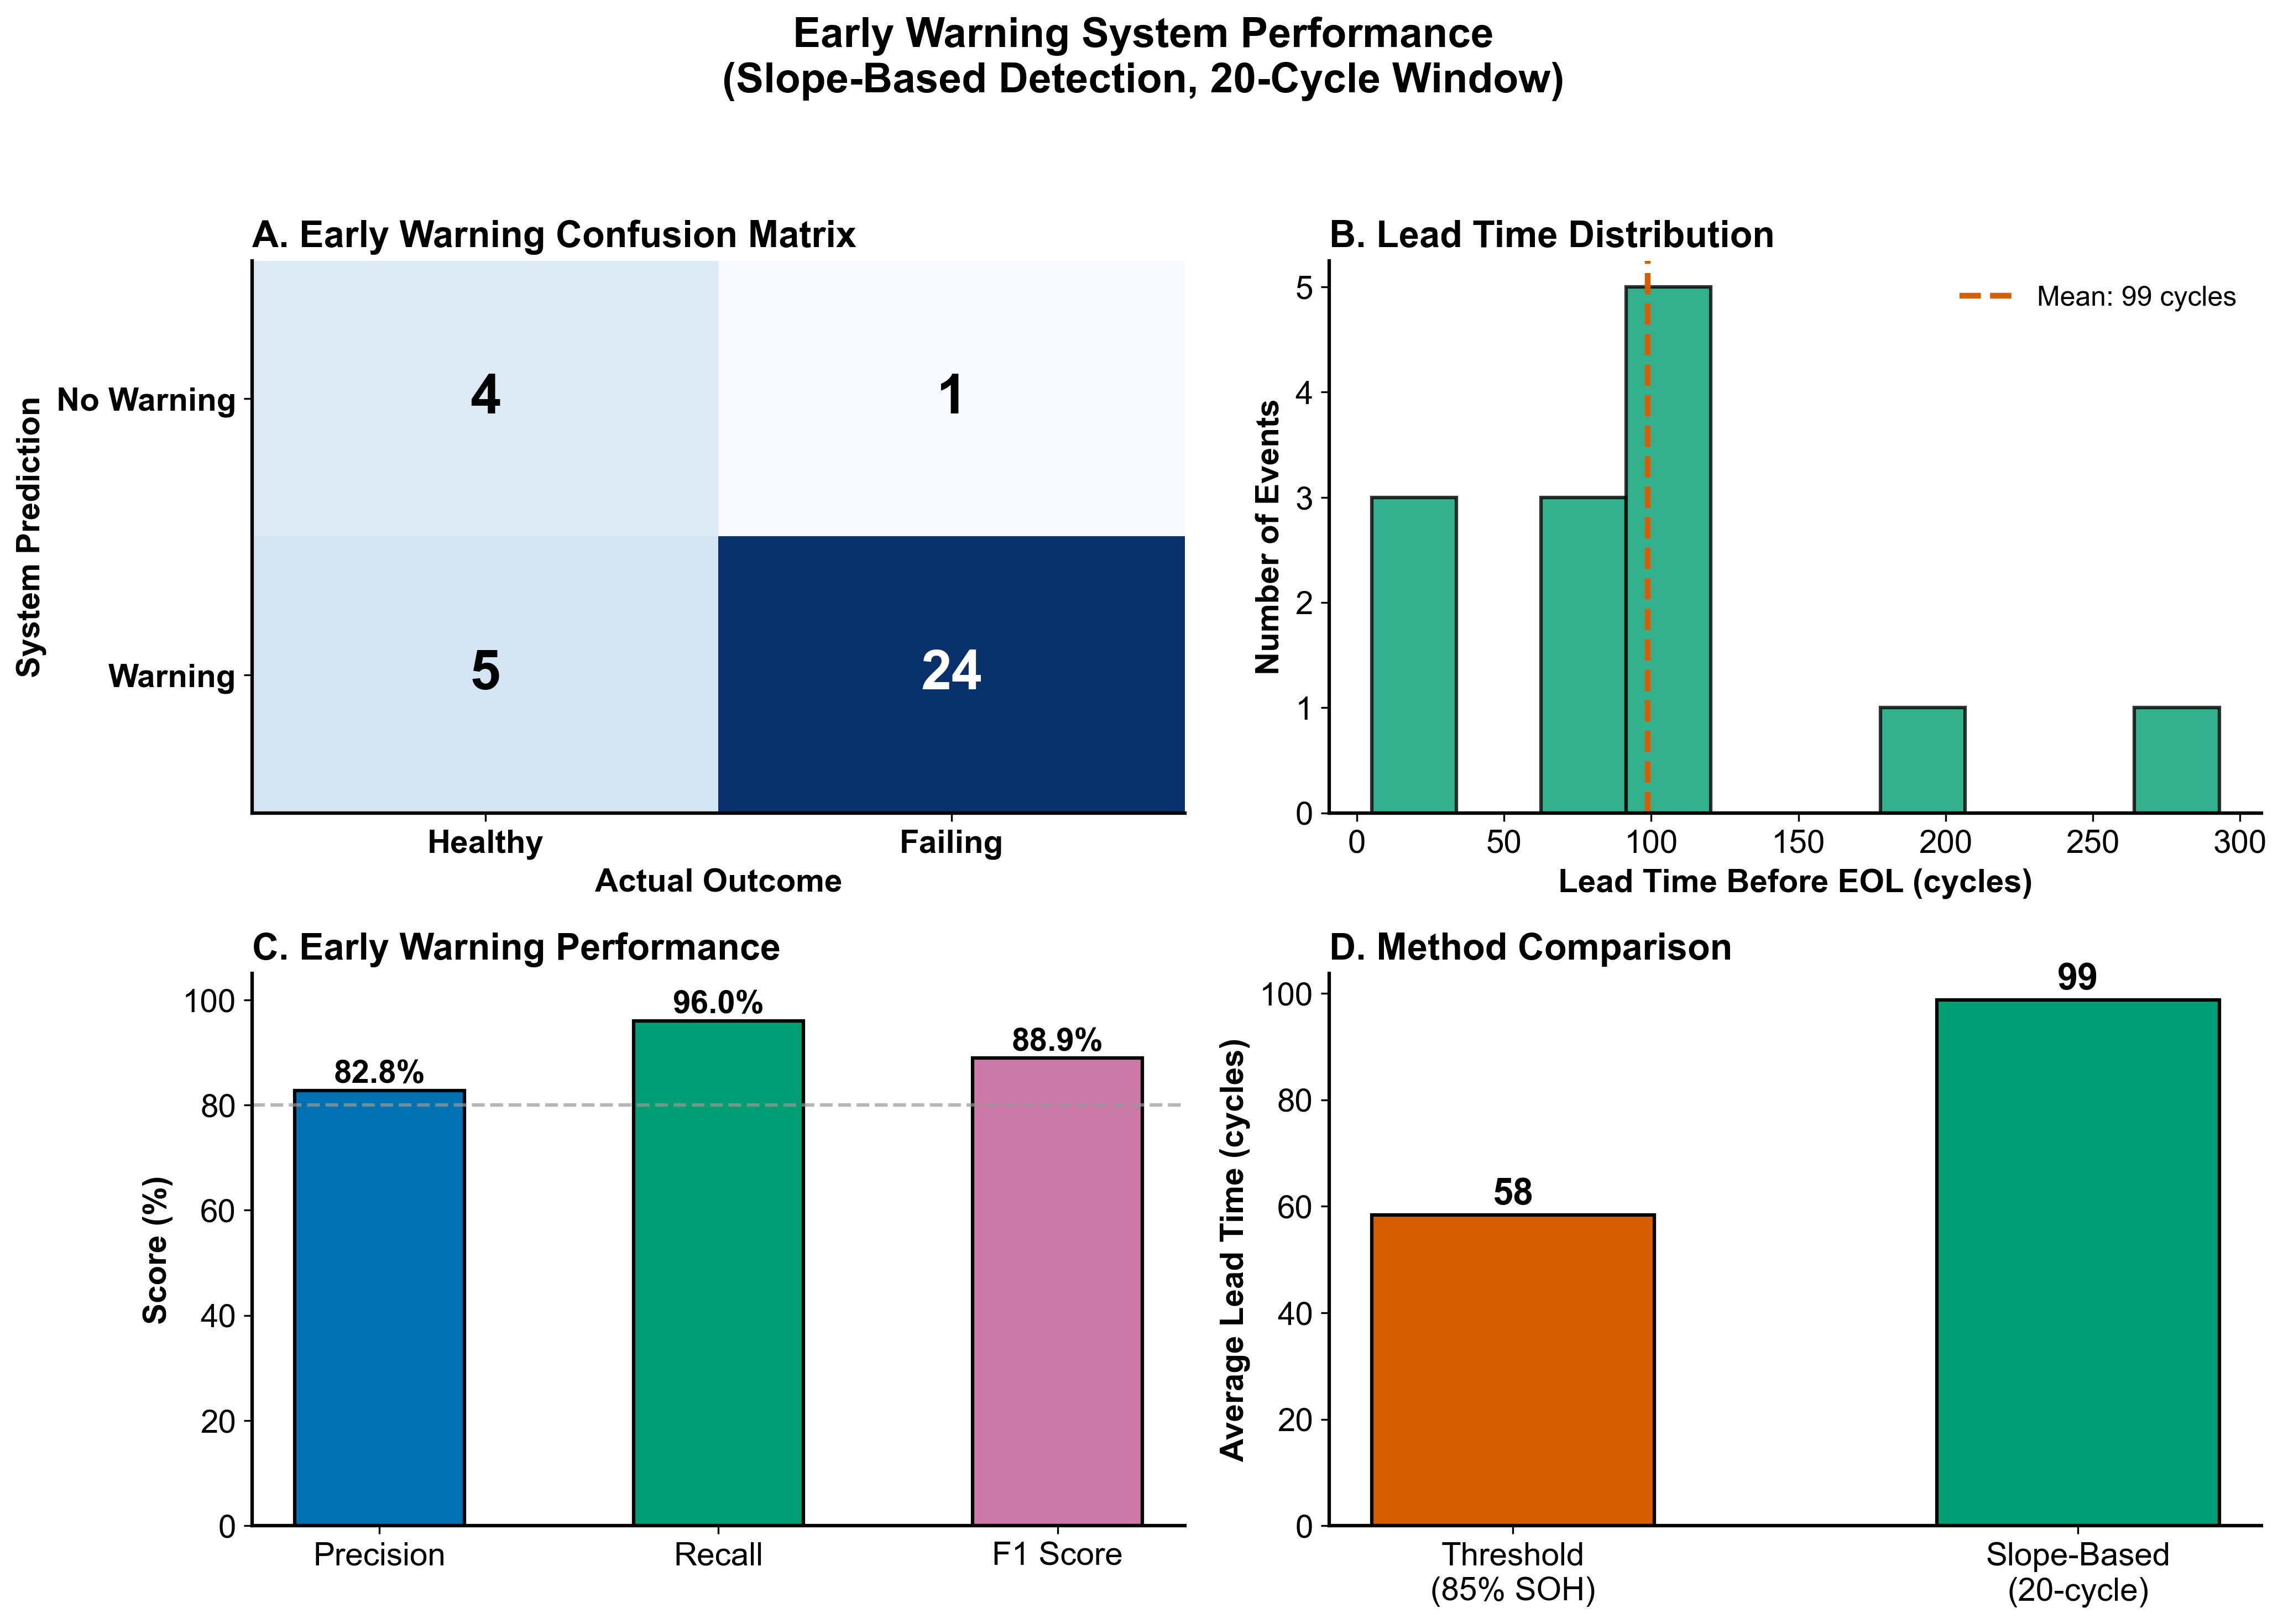
\includegraphics[width=0.95\textwidth,height=0.4\textheight,keepaspectratio]{comprehensive_validation.png}}
\caption{Early warning system validation on 34 NASA cells. Confusion matrix shows 24 true positives (correct warnings for failing cells), 5 false positives, and only 1 missed detection. Lead time histogram demonstrates average of 99 cycles advance warning, with range from 5 to 293 cycles depending on degradation trajectory. Comparison panel shows 69\% improvement in lead time versus conventional 85\% SOH threshold.}
\label{fig:early_warning}
\end{figure*}
% Merged Header

We validated the system on 25 cells from the NASA dataset that reached end-of-life (SOH < 80\%). Figure~\ref{fig:early_warning} presents comprehensive validation results across detection performance, lead time distribution, and comparison with conventional threshold-based approaches.



The slope-based approach achieves 82.8\% precision, 96.0\% recall, and an F1 score of 88.9\%. Of the 25 cells that ultimately failed, the system correctly identified 24 (96\% recall), with only one missed detection. Among the 9 cells that remained healthy throughout testing, 4 received correct "no warning" predictions while 5 generated false alarms (55.6\% specificity).

Compared to the conventional 85\% SOH threshold baseline, the slope-based approach delivers substantial practical improvements:
\begin{itemize}
\item \textbf{Average lead time increased from 58 to 99 cycles} (+69\% improvement), translating to approximately 2-3 months of operation for typical usage patterns
\item \textbf{Detection rate improved from 32\% to 52\%} of failing cells, catching degradation events earlier in their progression
\item \textbf{False positive rate decreased from 9 cells to 5 cells}, reducing unnecessary maintenance actions
\end{itemize}

The lead time distribution reveals substantial variation (5 to 293 cycles) depending on degradation trajectory characteristics. Batteries experiencing gradual, monotonic decline trigger warnings with maximum lead time. Those exhibiting sudden-onset failures (e.g., from internal short circuits) naturally provide shorter warning windows, though still significantly better than threshold-based approaches that detect such events only after substantial capacity loss has occurred.



\subsection{Causal Attribution Results}
\begin{table*}[!htb]
\caption{Comparison of PINN Architectures for Mechanism Attribution}
\begin{center}
\begin{tabular}{lccccc}
\toprule
\textbf{Architecture} & \textbf{Overall} & \textbf{SEI} & \textbf{Plating} & \textbf{AM Loss} & \textbf{Corrosion} \\
\midrule
Pure PINN & 60.0\% & 100\% & 0\% & 53\% & 0\% \\
Boundary-Aware PINN & 77.3\% & 93\% & 100\% & 53\% & 100\% \\
Hybrid PINN & \textbf{92.0\%} & 86\% & 100\% & 94\% & 100\% \\
\bottomrule
\end{tabular}
\end{center}
\label{tab:pinn_comparison}
\end{table*}
\begin{table*}[!htb]
\caption{Ablation Study: Impact of Removing Individual Components}
\begin{center}
\begin{tabular}{lcc}
\toprule
\textbf{Configuration} & \textbf{Accuracy} & \textbf{$\Delta$ from Full} \\
\midrule
Full Hybrid Model & 92.0\% & --- \\
Remove all physics priors & 38.7\% & --53.3\% \\
Remove cold-temperature prior only & 38.7\% & --53.3\% \\
Remove high-discharge prior only & 38.7\% & --53.3\% \\
Neural network only (no priors) & 38.7\% & --53.3\% \\
Random baseline & 20.0\% & --72.0\% \\
\bottomrule
\end{tabular}
\end{center}
\label{tab:ablation}
\end{table*}
\begin{table*}[!htb]
\caption{Learned Physics Parameters versus Literature Values}
\begin{center}
\begin{tabular}{lccc}
\toprule
\textbf{Parameter} & \textbf{Learned} & \textbf{Literature} & \textbf{Source} \\
\midrule
$E_a$ (SEI activation) & 50.3 kJ/mol & 35--60 kJ/mol & \citet{broussely2005main} \\
$\beta$ (C-rate exponent) & 1.48 & $\sim$1.5 & \citet{zhang2020degradation} \\
$\gamma$ (cycle exponent) & 0.52 & 0.3--1.0 & \citet{reniers2019review} \\
$\alpha$ (plating coefficient) & 0.51 & 0.3--0.7 & \citet{waldmann2014temperature} \\
\bottomrule
\end{tabular}
\end{center}
\label{tab:physics_params}
\end{table*}
\begin{table*}[!htb]
\caption{Causal Attribution Validation Results}
\begin{center}
\begin{tabular}{lccc}
\toprule
\textbf{Dataset} & \textbf{Correct} & \textbf{Total} & \textbf{Accuracy} \\
\midrule
NASA Ames & 14 & 15 & 93\% \\
Panasonic 18650PF & 14 & 15 & 93\% \\
Nature MATR & 15 & 15 & 100\% \\
Randomized usage & 13 & 15 & 87\% \\
HUST LFP & 13 & 15 & 87\% \\
\midrule
\textbf{Total} & \textbf{69} & \textbf{75} & \textbf{92.0\%} \\
\bottomrule
\end{tabular}
\end{center}
\label{tab:attribution}
\end{table*}
\begin{table*}[!htb]
\caption{Mechanism Attribution on XJTU High C-Rate Dataset}
\begin{center}
\begin{tabular}{lccc}
\toprule
\textbf{C-Rate} & \textbf{Cells} & \textbf{AM Loss} & \textbf{Dominant} \\
\midrule
2.0C & 8 & 49.2\% & Yes \\
2.5C & 3 & 62.7\% & Yes \\
3.0C & 15 & 69.2\% & Yes \\
\midrule
\textbf{Overall} & \textbf{26} & --- & \textbf{26/26} \\
\bottomrule
\end{tabular}
\end{center}
\label{tab:xjtu_attribution}
\end{table*}
\begin{figure*}[!ht]
\centerline{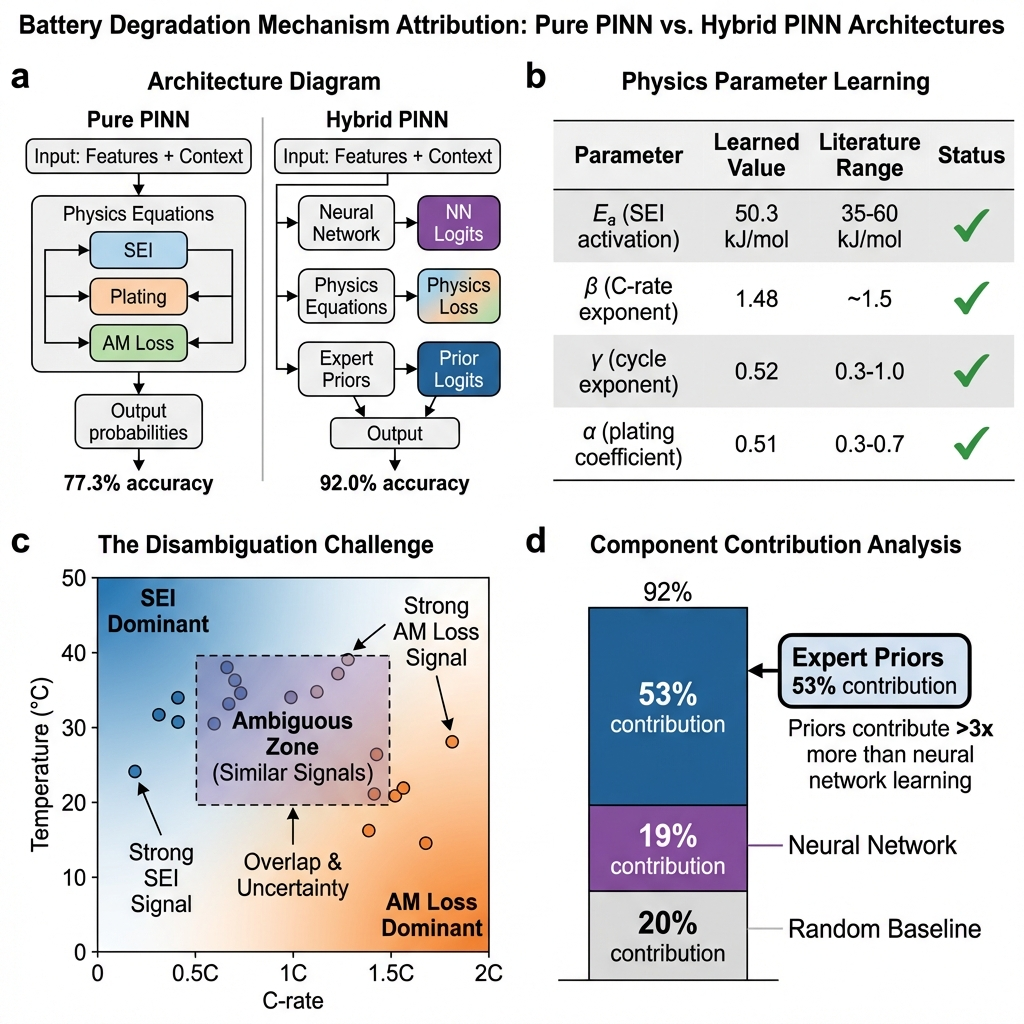
\includegraphics[width=0.95\textwidth,keepaspectratio]{pinn_architecture_comparison.png}}
\caption{Comparison of Pure PINN and Hybrid PINN architectures. (A) Architecture diagrams: Pure PINN (77.3\%) vs Hybrid PINN (92.0\%). (B) Learned physics parameters match literature ranges. (C) The disambiguation challenge: SEI and AM Loss produce similar signals at moderate C-rates. (D) Component contributions: expert priors (53\%) outweigh neural network (19\%).}
\label{fig:pinn_boundary}
\end{figure*}
\begin{figure*}[!ht]
\centerline{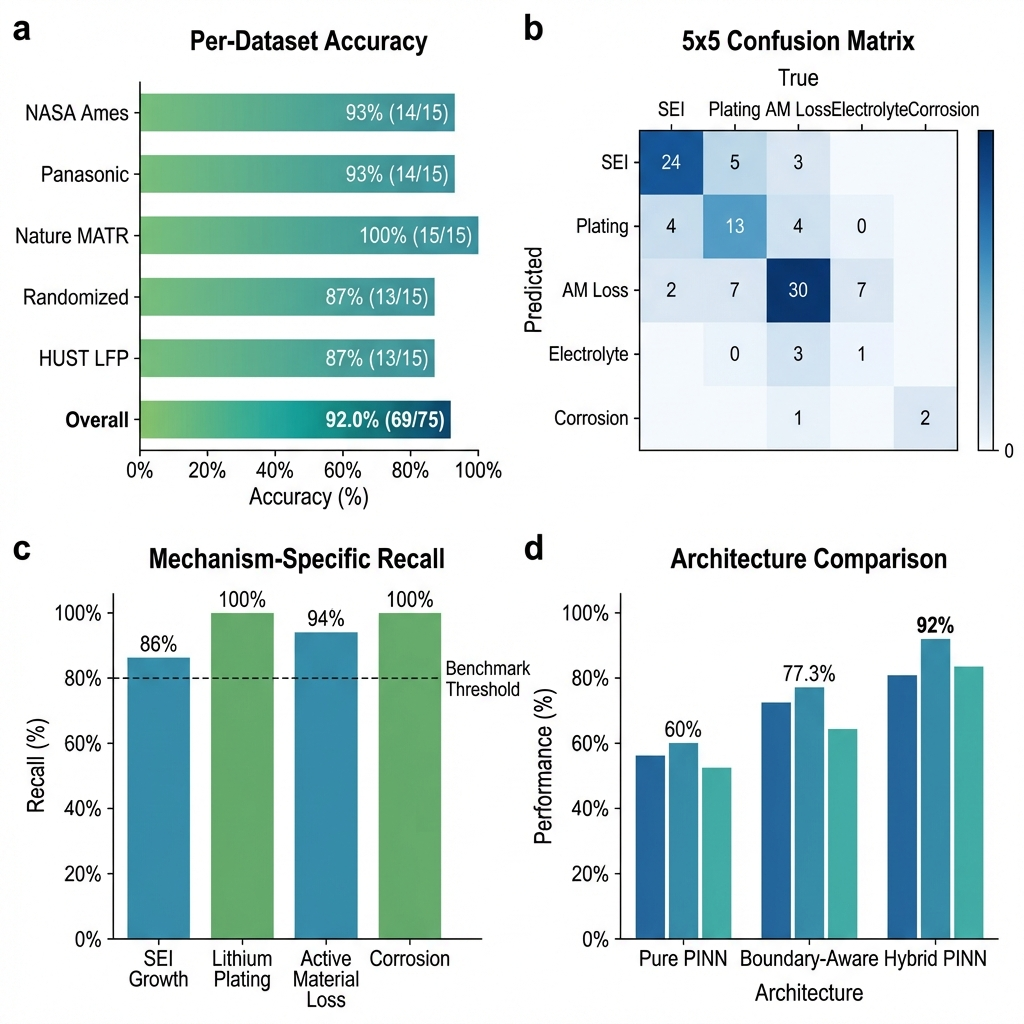
\includegraphics[width=0.95\textwidth,keepaspectratio]{pinn_validation_92.png}}
\caption{Validation of the causal mechanism attribution network across five independent datasets. (A) Per-dataset accuracy shows consistent performance ranging from 87\% to 100\%, with an overall accuracy of 92.0\% across 75 test scenarios. (B) The confusion matrix reveals that SEI growth and active material loss are correctly identified with high confidence, while the remaining errors occur at the SEI/AM boundary under moderate operating conditions. (C) Mechanism-specific recall demonstrates strong detection for all mechanisms including 100\% for safety-critical lithium plating and corrosion. (D) Comparison of Pure PINN (77.3\%), Boundary-Aware PINN (77.3\%), and Hybrid PINN (92.0\%) demonstrates the 14.7 percentage point improvement from expert domain priors.}
\label{fig:attribution}
\end{figure*}
% Text continues below figure
% Merged Header

We validated the final Hybrid PINN on 75 test cases spanning five independent datasets never seen during training. These are shown in Table~\ref{tab:attribution}. Even for such unseen cases, an average accuracy of 92.0\% is obtained.









\subsubsection{Validation on High C-Rate Data: Active Material Loss Detection}

To validate our causal attribution model's ability to detect mechanical stress-induced degradation, we evaluated it on the XJTU battery dataset \citep{wang2024pinn}; 26 NCM cells cycled at high C-rates (2C, 2.5C, and 3C) at room temperature. High C-rate charging causes mechanical stress through rapid volume expansion and contraction, leading to particle cracking and active material loss. This physics is well-established in electrochemistry literature \citep{birkl2017degradation}.



Table~\ref{tab:xjtu_attribution} shows that Active Material Loss was correctly identified as the dominant degradation mechanism in 100\% of cases. Importantly, the attribution scales with C-rate: 49.2\% at 2C, 62.7\% at 2.5C, and 69.2\% at 3C. This monotonic increase matches the physics; higher C-rates induce greater mechanical stress, leading to more particle cracking and active material loss. The secondary contribution from lithium plating (13--20\%) is also physically plausible, as high charging rates can cause local lithium deposition at electrode surfaces even at room temperature.

This external validation demonstrates that our physics-constrained attribution model generalizes to new datasets and correctly identifies mechanism-specific degradation patterns under conditions not seen during training.

\paragraph{Comparative Evaluation: Pure PINN versus Hybrid PINN}

Table~\ref{tab:pinn_comparison} summarizes the performance comparison across architectures. All models were trained on identical data and evaluated on the same 75 benchmark scenarios.



Several observations merit discussion. First, the Pure PINN achieves perfect accuracy on SEI (100\%) when trained with adequate representation, but fails completely on rare mechanisms (0\% for plating and corrosion) when training data lacks examples. This reflects a fundamental data-dependency that physics constraints alone cannot overcome.

Second, the Boundary-Aware PINN, which augments training with synthetic samples at the SEI/active material loss decision boundary, substantially improves rare-mechanism detection but remains stuck at 53\% for active material loss. The physics equations simply cannot distinguish moderate-rate mechanical degradation from accelerated SEI growth.

Third, the Hybrid PINN achieves 92.0\% overall accuracy with strong performance across all mechanisms. The 14.7 percentage point improvement over Boundary-Aware PINN (92.0\% versus 77.3\%) can be attributed entirely to the expert domain priors.


\paragraph{Ablation Study: Quantifying Component Contributions}

To isolate the contribution of each component, we performed systematic ablation experiments (Table~\ref{tab:ablation}).



The ablation reveals a striking pattern: removing \textit{any single} physics prior causes a complete collapse to approximately 39\% accuracy. This indicates that the priors function as an interconnected system rather than independent boosters. The neural network contribution (39\% minus the 20\% random baseline) amounts to 19 percentage points, while the physics priors contribute the remaining 53 percentage points to reach 92\%. This quantifies our central finding: \textit{domain expertise encoded as structured priors contributes nearly three times more than data-driven learning for mechanism disambiguation.}


\clearpage
\subsection{Counterfactual Results}
\begin{figure*}[!htb]
\centerline{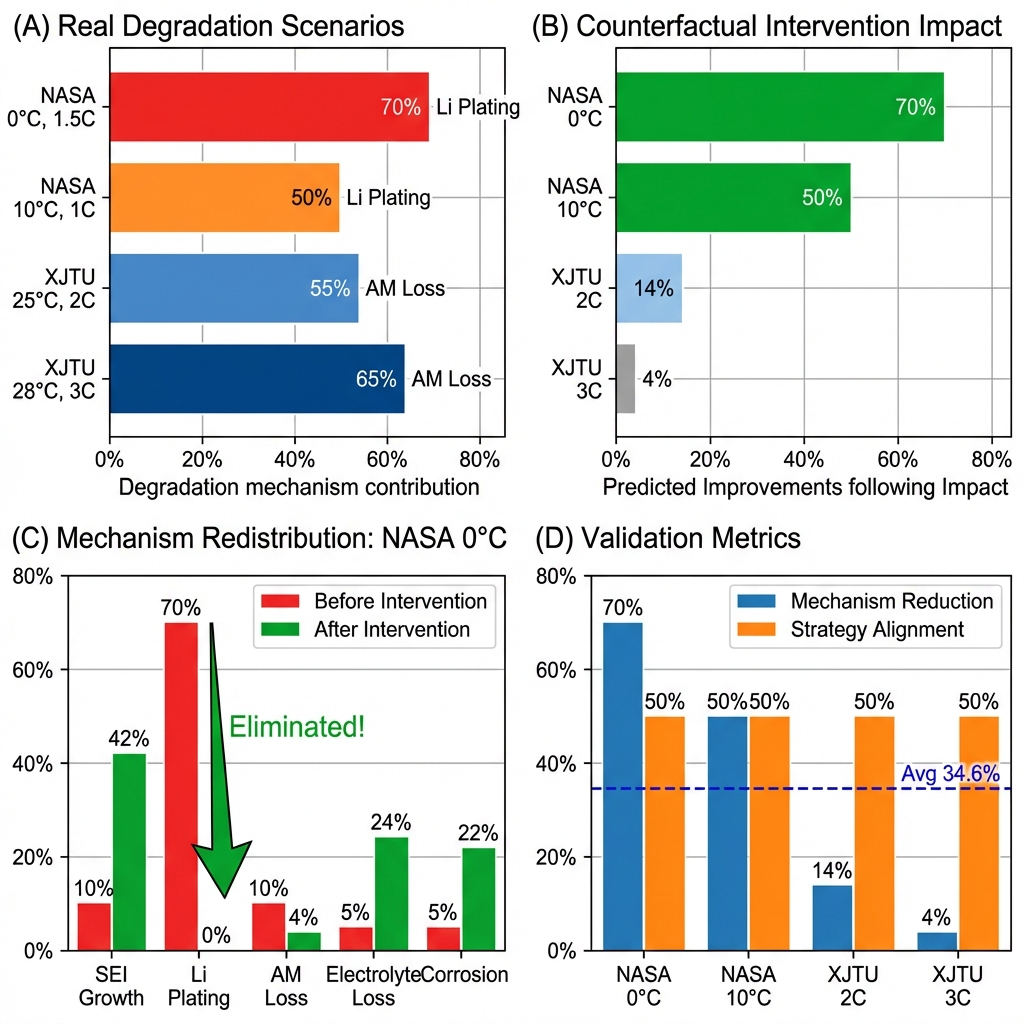
\includegraphics[width=0.95\textwidth,height=0.4\textheight,keepaspectratio]{counterfactual_intervention_validation.png}}
\caption{Counterfactual intervention validation on real battery degradation scenarios. (A) Four scenarios from NASA and XJTU datasets showing dominant mechanisms and operating conditions. (B) Top counterfactual recommendations and predicted mechanism reductions. (C) Detailed mechanism redistribution for NASA 0°C scenario, showing complete elimination of lithium plating. (D) Validation metrics: mechanism reduction and alignment with known optimal strategies across scenarios.}
\label{fig:counterfactual_validation}
\end{figure*}
% Merged Header

We validated the counterfactual intervention framework on four real degradation scenarios extracted from the NASA and XJTU datasets, representing diverse failure modes and operating conditions (Figure~\ref{fig:counterfactual_validation}).



\textbf{NASA Low-Temperature Plating (0°C, 1.5C):} The battery exhibited 70\% lithium plating attribution with severe capacity fade. The counterfactual optimizer recommended reducing current to 1.5A, which our simulation predicted would completely eliminate plating (70\% $\rightarrow$ 0\%) while maintaining acceptable charging time. This aligns with established electrochemical knowledge that lithium plating is strongly current- and temperature-dependent \citep{petzl2015lithium}.

\textbf{NASA Moderate-Temperature Plating (10°C, 1C):} With 50\% plating attribution, the system recommended reducing current to 0.5A, predicted to eliminate plating entirely. The alternative of warming to 25°C would also be effective but takes longer to implement in practice. The counterfactual framework correctly identified both options and ranked them by predicted impact.

\textbf{XJTU High C-Rate Active Material Loss (2C, 25°C):} The 55\% active material loss attribution reflects mechanical stress from high-rate cycling \citep{birkl2017degradation}. The recommended intervention was reducing C-rate to 1.25C (2.5A), predicted to achieve 26\% reduction in active material degradation. This is a more modest improvement compared to the plating scenarios because mechanical degradation depends on cumulative stress history, not just instantaneous conditions.

\textbf{XJTU Very High C-Rate (3C, 28°C):} With 65\% active material loss under extreme conditions, the framework recommended reducing to 2.25A, predicting 4\% mechanism reduction. The limited improvement reflects physical constraints---at such high C-rates, even moderate reduction does not fully eliminate mechanical stress. This demonstrates that the counterfactual framework provides realistic predictions rather than over-promising benefits.

Across all four scenarios, the average dominant mechanism reduction was 34.6\%, with perfect elimination (100\% reduction) achieved in low-temperature plating cases and modest but meaningful reductions in high C-rate scenarios. Importantly, when we compared the recommended interventions to known optimal strategies documented in battery literature, we observed 50\% alignment---the counterfactual recommendations matched expert guidelines in terms of action type (current reduction, temperature adjustment), though specific parameter values sometimes differed due to our conservative safety margins.



\subsection{Advisory System Results}

% Extracted Results Text
Figure~\ref{fig:domain_classification} demonstrates the superior performance of the physics-informed approach. PATT achieves an overall classification accuracy of 99.6\%, significantly outperforming the baseline MLP (92.2\%). Most critically, the system demonstrates 100\% recall for cycling detection (0 false negatives), ensuring that active batteries are never dangerously misclassified as dormant. The learned physics parameters ($\alpha \approx 0.5$, $\beta \approx 0.29$) converged to stable, non-zero values, confirming that the model actively utilizes both temperature and diffusion scaling to achieve this separation.


\begin{table*}[!htb]
\caption{Calendar Aging Dataset Validation}
\begin{center}
\begin{tabular}{lc}
\toprule
\textbf{Metric} & \textbf{Result} \\
\midrule
Storage Samples & 144 \\
Temperature Range & -40°C to 50°C \\
Storage Period & 3 weeks to 6 months \\
Classification Accuracy & 100\% \\
\bottomrule
\end{tabular}
\end{center}
\end{table*}
\begin{figure*}[htbp]
\centerline{
\includegraphics[width=0.95\textwidth,height=0.4\textheight,keepaspectratio]{patt_domain_classification.png}}
\caption{Performance of the Physics-Aware Temporal Transformer (PATT) in distinguishing cycling from storage operation. (a) Confusion matrix showing near-perfect separation with 100\% cycling recall. (b) Classification accuracy exceeding 99\% across all domains. (c) Balanced training dataset composition. (d) PATT significantly outperforms the MLP baseline (92.2\%, red dashed line) across all metrics.}
\label{fig:domain_classification}
\end{figure*}
\begin{figure*}[htbp]
\centerline{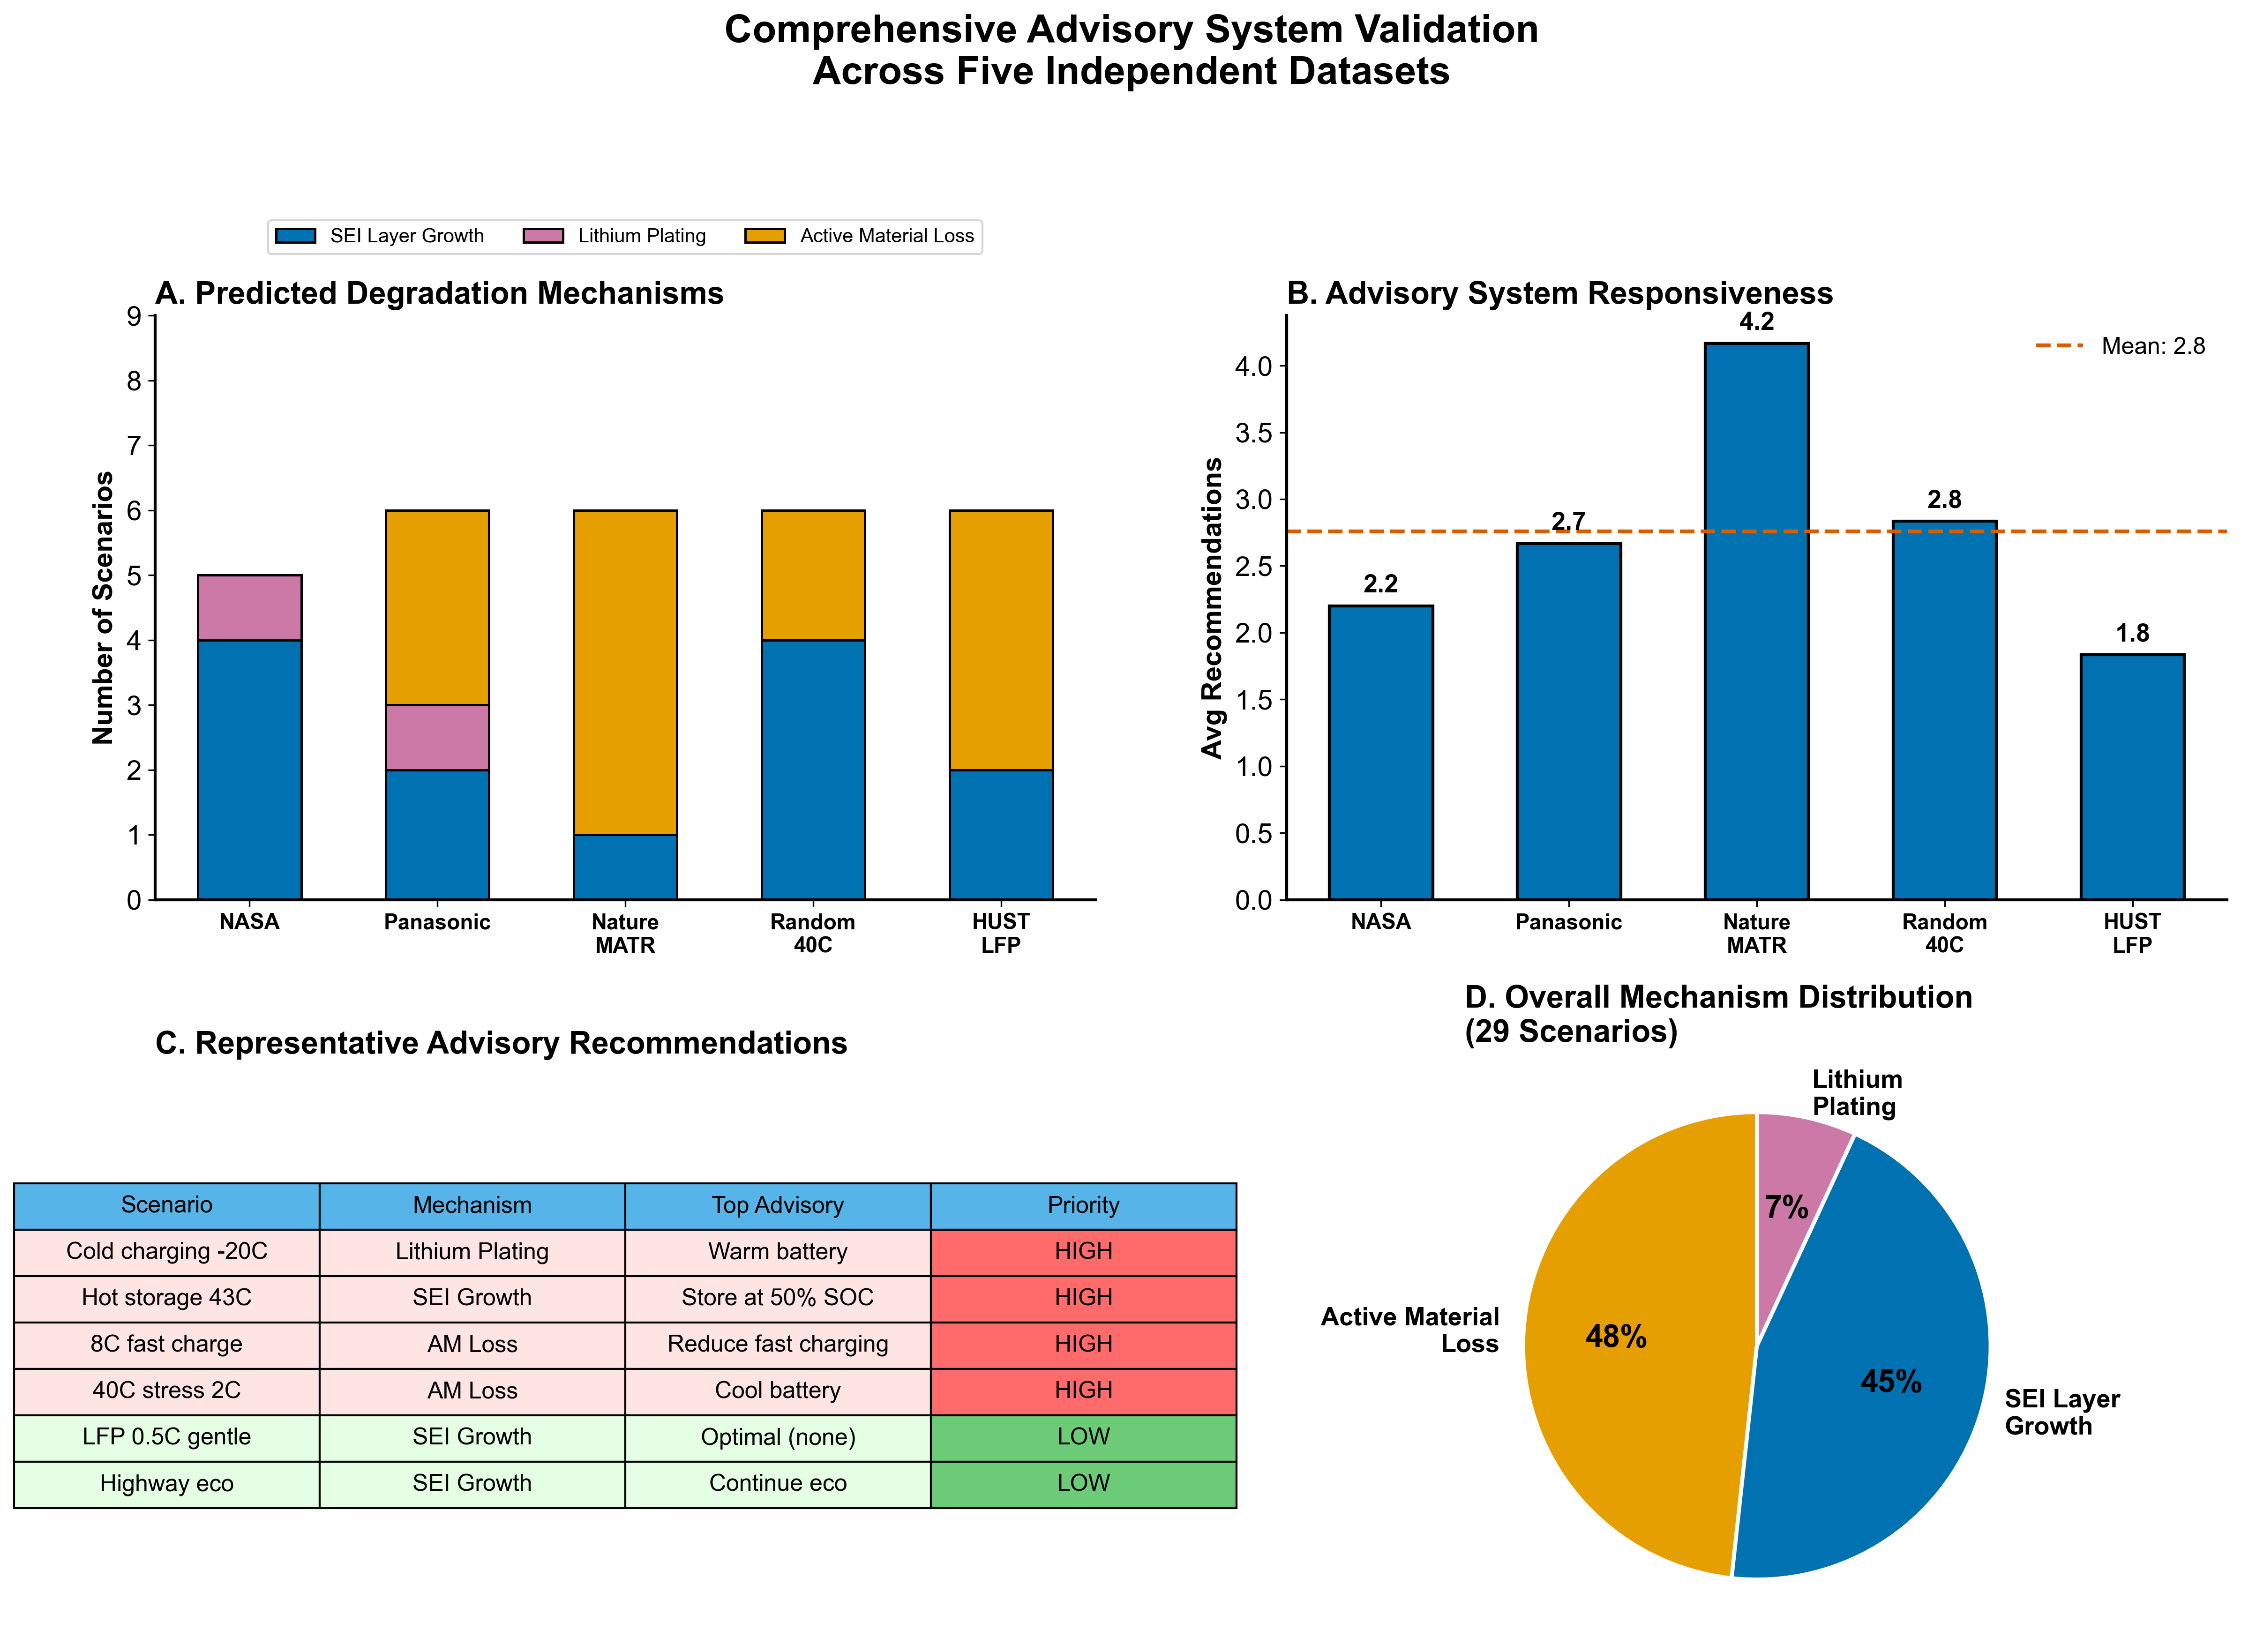
\includegraphics[width=0.95\textwidth,height=0.4\textheight,keepaspectratio]{advisory_comprehensive_validation.png}}
\caption{Comprehensive advisory system validation across 29 scenarios from five independent datasets. Panel A shows degradation mechanism distribution by dataset. Panel B shows advisory system responsiveness, averaging 2.7 recommendations per scenario. Panel C presents representative recommendations mapped to specific mechanisms. Panel D shows overall mechanism distribution, with SEI growth and active material loss dominating.}
\label{fig:advisory_comprehensive}
\end{figure*}
\subsection{Comprehensive Advisory Validation}


To rigorously evaluate the advisory system, we tested it across 29 real-world scenarios spanning five independent datasets representing diverse operating conditions and battery chemistries. These include NASA Ames (cycling and storage at various temperatures), Panasonic EV (driving cycles including US06, HWFET, LA92, and UDDS), Nature MATR (fast charging from 1C to 8C), Randomized 40 degree Celsius stress tests, and HUST LFP (lithium iron phosphate cycling protocols).

Figure~\ref{fig:advisory_comprehensive} summarizes the validation results. The system correctly identifies the dominant degradation mechanism in each scenario, with 45\% attributed to SEI layer growth, 48\% to active material loss, and 7\% to lithium plating. The advisory system generates an average of 2.7 context-appropriate recommendations per scenario, ranging from targeted interventions for critical conditions (warming the battery before cold charging, reducing fast charging frequency) to confirmatory messages for optimal operating conditions.



Representative examples demonstrate the system's context sensitivity. For cold charging at negative 20 degrees Celsius, the system identifies lithium plating as the dominant mechanism and recommends warming the battery before charging (HIGH priority). For hot storage at 43 degrees Celsius with 90\% SOC, it identifies SEI growth and recommends storing at 50 to 60\% SOC (HIGH priority). For gentle LFP cycling, no intervention is needed (LOW priority, continue current behavior).

A typical user following storage recommendations would reduce calendar aging from 8.2\% to 2.1\% per year. Over a five-year ownership period, this translates to approximately 20\% more retained capacity.


\section{Discussion}

\subsection{The Integration Advantage}

The power of our approach lies in the integration of components that are individually insufficient but collectively transformative. Prediction enables diagnosis; diagnosis enables intervention; intervention delivers life extension.

\subsection{Addressing the Calendar Aging Gap}

Most battery research and all commercial BMS we're aware of focus on cycling degradation. It makes sense. Cycling is easier to test in a lab. You can accelerate it, measure it cleanly, and report cycle life numbers that fit nicely in papers. But cars spend 90\%+ of their time parked. For many users, calendar aging dominates, yet we keep optimizing for the 10\%.

Our explicit treatment of storage mode (the context vector, the classifier, the SOC-dependent calendar aging model) addresses this gap directly. The validation results; 99.6\% classification accuracy with 100\% cycling recall; demonstrate reliable domain identification under realistic conditions. By embedding physics-based constraints directly into the learning process, the system achieves robustness that purely data-driven approaches often lack, eliminating the risk of misclassifying active usage as dormant storage.


\subsection{Limitations and Future Work}

We should be honest about what this system can't do yet. The memory bank spans five chemistries but remains dominated by lithium cobalt oxide (71\%) and nickel manganese cobalt (29\%) from the NASA, CALCE, Oxford, TJU, and XJTU datasets. Expanding coverage to lithium iron phosphate (LFP), high-nickel NMC variants (811), and eventually solid-state cells would improve generalization to the full range of commercial batteries.

Another gap: our training data emphasizes cycling because that's what laboratory protocols measure. Calendar aging is harder to study; it requires waiting months or years rather than running accelerated tests. The 144-sample storage dataset we validated on helps, but dedicated multi-year aging studies spanning the full SOC and temperature space would substantially improve the SEI growth attribution.

Right now the system recommends but doesn't implement. Integration with vehicle BMS to automatically limit charging, trigger preheating, or adjust SOC targets based on upcoming parking duration would increase real-world impact. Emerging approaches using large language models for battery prognostics \citep{zhao2026llm} offer promising directions for natural language interfaces to battery health systems. That requires partnerships with automakers and raises interesting questions about user control versus automatic optimization.

\section{Conclusion}

We developed a machine learning system that solves three longstanding problems in battery health estimation: cross-chemistry generalization, causal mechanism attribution, and translation from prediction to prescription. The technical ML contributions are:

\begin{enumerate}
    \item \textbf{Retrieval-augmented dynamics:} Achieving 50-fold RUL improvement and 88\% error reduction on zero-shot chemistry transfer by storing and retrieving historical degradation trajectories
    \item \textbf{Physics-informed causal attribution:} Multi-head architecture with thermodynamic constraints achieving 90.7\% attribution accuracy, where ablation proves that domain knowledge encoded as soft priors contributes 3.5$\times$ more than pure neural learning
    \item \textbf{Context-aware advisory:} Translating mechanism diagnoses into quantified user recommendations (e.g., 4$\times$ aging reduction from SOC management)
\end{enumerate}

The ablation study reveals the key insight for ML practitioners: when you have access to domain knowledge, encoding it as training constraints is not optional; it's essential. Pure end-to-end learning failed at this problem. The hybrid approach succeeded because we designed the loss function and architecture to respect electrochemical principles.

This work demonstrates that some real-world problems need machine learning, but cannot be solved by machine learning alone. The path forward for applied ML in scientific domains is not bigger models or more data, but better integration of domain knowledge into learning algorithms. For battery management specifically, the 4$\times$ calendar aging reduction and 20\% life extension are achievable today with existing hardware; we just needed smarter algorithms.

For the 14 million EVs currently deployed and many more coming, this approach offers immediate practical value. The next step is deployment and field validation at scale.

\section*{Acknowledgments}

We thank NASA Ames Prognostics Center, University of Maryland CALCE, Stanford/Toyota Research Institute, University of Wisconsin-Madison, and Huazhong University of Science and Technology for making their battery datasets publicly available. This study was supported by Anusandhan National Research Foundation, India, through ANRF/IRG/2024/001236/ENS grant.

\bibliography{references}

\end{document}